\chapter{Circumventing Undersegmentation - GMM for Conservation Tracking}
\label{cha:GMM}

While the conservation tracking (\cref{subsec:fg-conservation}) is capable of detecting merged
objects and inferring the number of cells per connected component, the factor graph by itself has no
means for separating merged objects and thus reconstructing lost tracks.  Even with the knowledge of
merged objects, tracks will be lost, including division events. This may, depending on the number of
merged objects in the segmentation, heavily deteriorate the tracking result -- a downgrade that can
be evaded given the knowledge about merged objects.

In order to reconstruct the lost tracks, we introduce a two-step post-processing procedure on the
conservation tracking result depicted in \cref{fig:gmm-pipeline}:
\begin{enumerate}
      \item Reconstruct cells for all connected components that contain more than one cell according
    to the conservation tracking.
      \item Build a hypotheses graph on this subset of cells and rerun the tracking with new
    constraints, ensuring that \label{itm:gmm-new-constraints}
    \begin{enumerate}
          \item all cells are active, and \label{itm:gmm-all-cells-active}
          \item no divisions occur. \label{itm:gmm-no-divisions}
    \end{enumerate}
\end{enumerate}

\begin{figure}
    \centering
    \begin{tikzpicture}
        % \begin{scope}[every node/.append style={yslant=0.5,xslant=-1},yslant=0.5,xslant=-1]
        \node[anchor=south west,inner sep=0] (image) at (0,0)
        {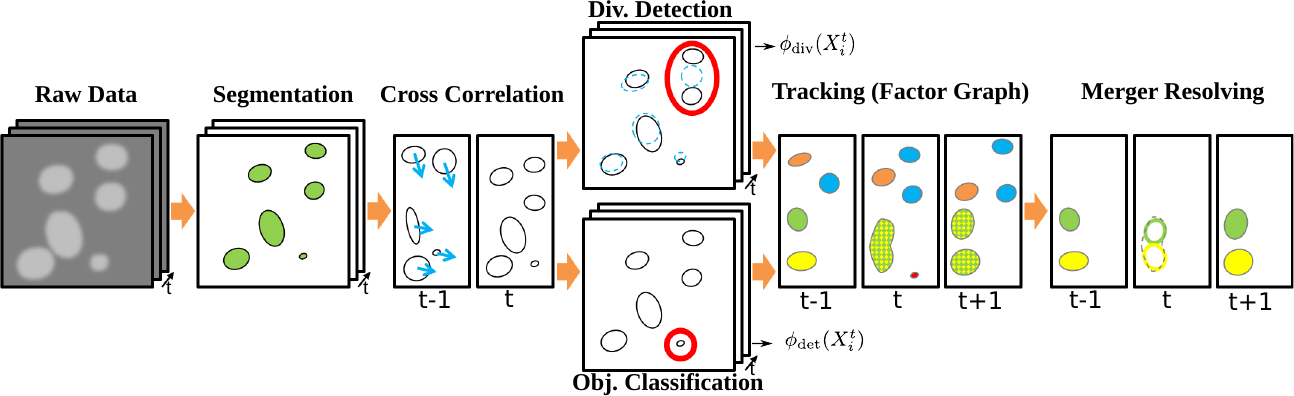
\includegraphics[width=\textwidth]{images/gmm/pipeline.png}};
        \begin{scope}[x={(image.south east)},y={(image.north west)}]
            \draw[red,line width=2pt,rounded corners, fill=red!20, fill opacity=0.3] (0.81,0.20) rectangle (1.003,0.81);
        \end{scope}
    % \end{scope}
    \end{tikzpicture}
    % \rule{\textwidth}{0.3pt}
    \caption[Conservation tracking pipeline including merger resolution]{New conservation tracking
        pipeline (taken from~\cite{schiegg_13_conservation}): \cref{fig:fg-conservation-pipeline} is
    extended by the merger resolution post-processing as indicated by the red rounded rectangle.}
\label{fig:gmm-pipeline}
\end{figure}

With evidence about the number of cells per connected component, unsupervised clustering algorithms
are a viable choice for cell reconstruction. The key feature to be reconstructed is the center of
mass for each cell as it is needed for both the creation of the new hypotheses graph and inference
in order to deduct the tracking result, corrected for mergers. More precisely, it is valid to assume
that the ellipsoidal shape of cells can be matched to covariance matrices of Gaussian
distributions. This is in contrast and preferable to the k-means clustering
algorithm\citep{macqueen_67_methods}. Therefore, \emph{Gaussian mixture models} (GMMs) are a viable
choice for such a task, with implementations readily available.

The new constraints which constrict inference on the subset hypotheses graph are a direct result of
the method being a post-processing for conservation tracking: The conservation tracking factor graph
infers the correct number of cells in the respective connected components and conservation of mass
enforces that these numbers are consistent over time. Furthermore, no divisions may, because the
conservation tracking disallows divisions cooccuring with mergers. Reintroducing divisions in the
post-processing method would require deactivating cells, in order to allow for global consistency,
which is vetoed by prerequisite that the number of cells in a connected component is correct.

In the following, we show how Gaussian mixture models can be utilized for cell reconstruction in
\cref{sec:gmm-gmm}, before describing the construction of the new hypotheses graph on the subset
of cells and the inference of the final tracking solution in \cref{sec:gmm-hypotheses}. Finally,
the experiments in \cref{sec:gmm-experiments} show results of the proposed method.

\section{Gaussian Mixture Models and Cell Reconstruction}
\label{sec:gmm-gmm}
Data that form \emph{clusters} in feature space, \ie regions with a dense accumulation of
data points, can be meaningfully interpreted as data generated by a distribution with multiple
local maxima, which, in turn, can be modeled by a convex combination of simpler, single-mode distributions.

\begin{mydef}
    \label{def:convex-combination}
    A \emph{convex combination} of points $\{x_h\}_{h=1,\hdots,H}$ is a linear combination of points
    $\{x_h\}_{h=1,\hdots,H}$ with non-negative weights $\{\alpha_h\}_{h=1,\hdots,H}$ that sum up to $1$ (normalization):
    \begin{align}
        \label{eq:def-convex-combination}
        &\sum_{h=1}^H \alpha_h x_h, \\
        &\alpha_h \ge 0 \; \forall h \wedge \sum_{h=1}^H \alpha_h = 1.
    \end{align}
\end{mydef}
For clarification, the convex combination of the unit coordinate vectors in three dimensions is visualized in
\cref{fig:gmm-convex-combination}.
\begin{figure}
    \centering
    \tdplotsetmaincoords{60}{110}

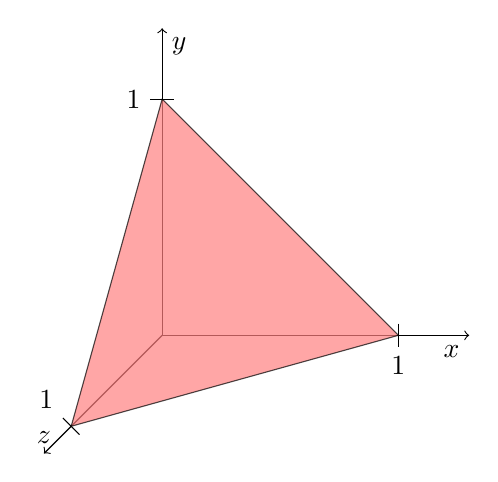
\begin{tikzpicture}[scale=3]
    \begin{scope}
        \draw[->] (0,0,0) -- (1.3,0,0) node[anchor=north east]{$x$};
        \draw[->] (0,0,0) -- (0,1.3,0) node[anchor=north west]{$y$};
        \draw[->] (0,0,0) -- (0,0,1.3) node[anchor=south]{$z$};
        \draw [fill=red!50, opacity=0.7] (0,0,1)--(1,0,0)--(0,1,0)--cycle;
        \draw (1,0.05,0) -- (1,-0.05,0) node[anchor=north]{$1$};
        \draw (0.05,1,0) -- (-0.05,1,0) node[anchor=east] {$1$};
        \draw (0.035,-0.035,1) -- (-0.035,0.035,1) node[anchor=south east]{$1$};
        
    \end{scope}
\end{tikzpicture}

%%% Local Variables: 
%%% mode: latex
%%% TeX-master: "../../main"
%%% End: 

    %\rule{\textwidth}{0.3pt}
    \caption[Convex sum visualization]{A visualization of the convex sum of unit vectors in a three dimensional coordinate
        system: The red area (including the boundary) is the feasible region for the convex combination.}
    \label{fig:gmm-convex-combination}
\end{figure}

\cref{def:convex-combination} allows for definition of \emph{mixture models} in terms of convex
combinations.
\begin{mydef}[{{\citealp[Chapter~20]{barber_12_bayesian}; \citealp[Chapter~9]{bishop_07_pattern};
            \citealp{mclachlan_00_finite}}}]
    \label{def:mixture-model}
    A convex combination of distributions\footnote{The term ``distribution'' here refers to probability density~\citep[158]{barber_12_bayesian}.}
    \begin{align}
        \label{eq:gmm-distribution}
        p(v) = \sum_{h=1}^Hp(v|h)p(h)
    \end{align}
    is called a \emph{mixture model}.
\end{mydef}
The \emph{visible} variable $v$ corresponds to a data sample. The distribution is a sum of $H$
component models $p(v|h)$ weighted by $p(h)$, which corresponds to the weight $\alpha_h$ in
\cref{eq:def-convex-combination}. The weight can be interpreted as the prior probability of the data
sampled being generated by a particular component $h$, representing cluster $h$, as the definition
of a convex combination fulfills the requirements of a discrete probability distribution, namely
non-negativity and normalization. The data generation process follows a two step procedure: First, a
component distribution index $h$ is sampled from $p(h)$. Then, a data point is sampled from
$p(v|h)$. $h$ is called a \emph{hidden} variable.

In a \emph{Gaussian mixture model}, the data follow a convex sum of multivariate Gaussian distributions,
\begin{align}
    \label{eq:gmm-normal}
    p(v|h) &= \mathcal{N}({v}|\MUH , \SIGMAH ) \\ 
    &= \frac{1}{\sqrt{\det(2\pi\SIGMAH )} }\exp\left(-\frac{1}{2}({v}-\MUH )^\intercal
        \left(\SIGMAH\right) ^{-1} ({v}-\MUH )\right),
\end{align}
with mean $\MUH$ and covariance matrix $\SIGMAH$ for each component $h$. In general,
\begin{align}
    z\sim\mathcal{N}(z|\mu, \Sigma)
\end{align}
denotes that variable $z$ follows a normal distribution with
mean $\mu$ and covariance $\Sigma$. For brevity,
\begin{align}
    \label{eq:gmm-theta}
    \Theta &= \left\{\THETAH\right\}_{h=1,\hdots ,H}, \\
    \THETAH &= \left\{\MUH, \SIGMAH\right\}
\end{align}
refer to all parameters of the $h$-th component of the Gaussian mixture model. The parameters
\begin{align}
    \label{eq:gmm-pi}
    \Pi &= \left\{\pi_h\right\}_{h = 1, \hdots , H}, \\
    p(h) &= \pi_h \; \forall h \label{eq:gmm-pi-2}
\end{align}
define the discrete probability distribution to weigh the cluster components. \cref{fig:gmm-example}
shows data sampled from two Gaussian distributions and a GMM fit to the data.

\newsavebox{\covmatfirst}% Box to store smallmatrix content
\savebox{\covmatfirst}{$\left(\begin{smallmatrix}\hfill 5.25&\hfill 1.575\\\hfill 1.575&\hfill 3.5\end{smallmatrix}\right)$}
\newsavebox{\covmatsecond}% Box to store smallmatrix content
\savebox{\covmatsecond}{$\left(\begin{smallmatrix}\hfill 2.8&\hfill 1.75\\\hfill 1.75&\hfill 5.95\end{smallmatrix}\right)$}
\newsavebox{\predmatfirst}% Box to store smallmatrix content
\savebox{\predmatfirst}{$\left(\begin{smallmatrix}\hfill 5.16&\hfill 1.53\\\hfill 1.53&\hfill 3.41\end{smallmatrix}\right)$}
\newsavebox{\predmatsecond}% Box to store smallmatrix content
\savebox{\predmatsecond}{$\left(\begin{smallmatrix}\hfill 2.86&\hfill 1.87\\\hfill 1.87&\hfill 5.89\end{smallmatrix}\right)$}

\begin{figure}
    \centering
    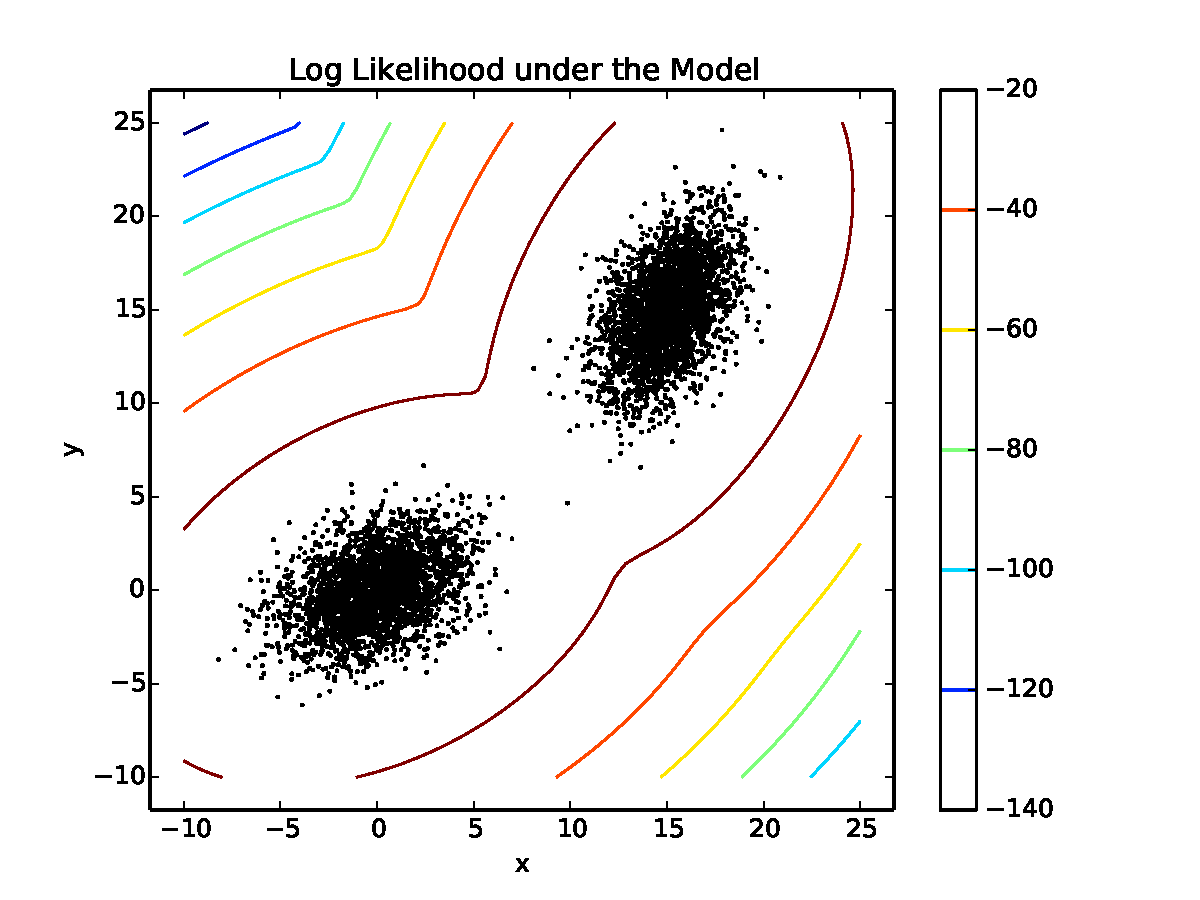
\includegraphics[width=0.7\textwidth]{images/gmm/gmm_example.pdf}
    %\rule{\textwidth}{0.3pt}
    \caption[GMM example]{\protect The black circles are data points sampled from two normal distributions with
        $\mu_1=(0,0)^\intercal$,$\Sigma_1=$\usebox{\covmatfirst} and
        $\mu_2=(15,15)^\intercal$,$\Sigma_2=$\protect\usebox{\covmatsecond}. 3000 samples are taken from
        each distribution. The GMM fit is represented by colored contour lines that represent levels
        of equal observation log likelihood. The predicted parameters are $\mu_1^{pred}=(-0.03,
        0.02)^\intercal$,$\Sigma_1^{pred}=$\protect\usebox{\predmatfirst}, $\mu_2^{pred}=(15.02,
        14.99)^\intercal$,$\Sigma_2^{pred}=$\protect\usebox{\predmatsecond}. The prior probabilities are in
        accord with the data generation process $\pi_1 = \pi_2 =
        0.500$.}
        % Scikit-learn~\cite{scikit-learn} and Matplotlib~\cite{hunter_07_matplotlib} were
        % used to create this plot.
        % $\sigma_1=\left(
        %     \begin{smallmatrix}
        %         1.5 &-0.9 \\
        %         0 & 1
        %     \end{smallmatrix}
        %     \right)$
    \label{fig:gmm-example}
\end{figure}

For $N$ independent and
identically distributed (\emph{iid}) random variables $\{v^n\}_{n=1,\hdots ,N}$, a Gaussian mixture model takes the form
\begin{align}
    \label{eq:gmm-iid}
    p(v^1,\dots ,v^N, h^1, \dots ,h^N) = \prod_{n=1}^N p(v^n|h^n)p(h^n).
\end{align}
Here, $h^n \in \{1,\hdots ,H\}$ means that the $n$-th data sample is assigned to cluster $h^n$.  A
graphical representation of this distribution is shown in \cref{fig:gmm-gm-plate} using the plate
notation:
\begin{mydef}
    In the visual representation of graphical models, \emph{plate notation} refers to grouping
    variables into a subgraph by enclosing them in a rectangle (plate). The number on the plate is
    the number of repetitions or duplications of that subgraph.
\end{mydef}
An illustrative example for plate notation is given in \cref{fig:gmm-plate-expl}.
\begin{figure}
    \centering
    \begin{subfigure}[t]{0.48\textwidth}
        \centering
        \begin{tikzpicture}[baseline=0pt]
    \begin{scope}
        \node[main, label=below:$v_1$, fill=black!30] (v) {};
        \node[main, label=below:$v_2$, fill=black!30, above of=v] (v1) {};
        \node[main, label=below:$v_3$, fill=black!30, below of=v] (v2) {};
        \node[main, label=below:$h$, left of=v, xshift=-10] (h) {};
        \path (h) edge[connect] (v);
        \path (h) edge[connect] (v1);
        \path (h) edge[connect] (v2);
    \end{scope}
\end{tikzpicture}


%%% Local Variables: 
%%% mode: latex
%%% TeX-master: "../../main"
%%% End: 

        \caption{Directed Acyclic Graph}
        \label{fig:gmm-plate-expl-dag}
    \end{subfigure}
    ~
    \begin{subfigure}[t]{0.48\textwidth}
        \centering
        \begin{tikzpicture}[baseline=0pt]
    \begin{scope}
        \node[main, label=below:$v$, fill=black!30] (v) {};
        \node[main, label=below:$h$, left of=v, xshift=-10] (h) {};
        \node[main, fill=black!30, below of=v, color=black!0] (v2) {};
        \node[rectangle, inner sep=5mm,draw=black!100, fit= (v)] (r) {};
        \node[anchor=south east,inner sep=1pt] at (r.south east) {$3$};
        \path (h) edge[connect] (v);
        %%%% DIRTY HACK TO ALLOW FOR CAPTIONS BEING ON THE SAME HEIGHT!!
        %%%% MAYBE RECONSIDER!!
        \node[main, label=below:{\color{white} 1}, color=black!0, fill=black!0, below of=v] (v2) {};
    \end{scope}
\end{tikzpicture}

%%% Local Variables: 
%%% mode: latex
%%% TeX-master: "../../main"
%%% End: 

        \caption{Plate Notation}
        \label{fig:gmm-plate-expl-plate}
    \end{subfigure}
    %\rule{\textwidth}{0.3pt}
    \caption[Plate notation example]{Plate notation example: The distribution $p(v_1,v_2,v_3,h) =
        p(v_1|h)p(v_2|h)p(v_3|h)p(h)$ is represented by a directed acyclic graph
        (\subref{fig:gmm-plate-expl-dag}). The plate notation for the same graph in
        (\subref{fig:gmm-plate-expl-plate}) is much  more compact.}
    \label{fig:gmm-plate-expl}
\end{figure}
The observation likelihood for given data can be derived by marginalizing over \cref{eq:gmm-iid}:
\begin{align}
    \label{eq:gmm-obs-likelihood}
    p(v^1,\hdots ,v^N) = \prod_{n=1}^N\sum_{h^n=1}^Hp(v^n|h^n)p(h^n).
\end{align}
For the application of GMMs in the context of conservation tracking, it is mandatory to infer the
cluster a data point belongs to. This can be achieved by maximizing the conditional probability
\begin{align}
    \label{eq:gmm-assign-clusters}
    \left\{ h_{\max }^n\right\}_{n=1,\hdots ,N} = &\argmax_{ h^1, \hdots ,h^N} p(h^1, \dots ,h^N|v^1,
    \hdots ,v^N) \\
    = & \left\{ \argmax_{h^n} p(h^n|v^n) \right\}_{n=1,\hdots ,N}.
\end{align}
The second equality holds due to the factorization of the distribution.  For this operation, the
model parameters $\Theta$ and $\Pi$ as defined in \crefrange{eq:gmm-theta}{eq:gmm-pi-2} need to be determined first, which
requires a formulation of the distribution that explicitly shows the dependency on the model
parameters:
\begin{align}
    \label{eq:gmm-distr-param}
    p(v^1,\dots ,v^N,h^1,\dots h^N|\Theta ,\Pi ) = \prod_{n=1}^Np(v^n|h^n, \Theta )p(h^n|\Pi )
\end{align}
The optimal parameters
\begin{align}
    \label{eq:gmm-ml}
    \left\{\Theta_{opt} ,\Pi_{opt}\right\} &= \argmax_{\Theta ,\Pi } p\left(v^1,\hdots ,v^N|\Theta
        ,\Pi\right) \\
    &= \argmax_{\Theta ,\Pi } \prod_{n=1}^Np\left(v^n|\Theta ,\Pi\right)
\end{align}
are then inferred by maximum likelihood. The commonly-used method for maximizing the likelihood of a
mixture model is the \emph{expectation maximization} (EM) algorithm, an iterative procedure, that in
many cases, including Gaussian mixture models, results in simple update formulae for the model
parameters. In general, the EM algorithm consists of an iterative repetition of two steps, namely the
\begin{itemize}
      \item \textbf{E-step} that maximizes the likelihood for the current set of parameters, \ie -- in
    the case of clustering -- assigning the data points to the correct clusters, and the
      \item \textbf{M-step} that -- given the assignments from the E-step -- estimate the parameters
    of the distribution.
\end{itemize}
These two steps are repeated until convergence or an iteration threshold. In general and in
particular for the Gaussian mixture models, the likelihood
is not a convex function. Therefore, the EM algorithm might get stuck in local minima and the result
can vary depending on the initial parameters. Detailed explanations of the EM algorithm can be
found in \citep[Chapter~11.2]{barber_12_bayesian},
\citet[Chapter~3]{mclachlan_97_em} and \citet{borman_04_expectation}.

The update equations for EM on a Gaussian mixture models are:
\begin{align}
    \label{eq:gmm-update-eq}
    \MUH_{\text{new}} &= \sum_{n=1}^Np_{\text{old}}\left(v^n|h\right)v^n, \\
    \SIGMAH_{\text{new}} &=
    \sum_{n=1}^Np_{\text{old}}(v^n|h)\left(v^n-\MUH\right)\cdot\left(v^n-\MUH\right)^\intercal, \\
    p_{\text{new}}(h) &= \frac{1}{N}\sum_{n=1}^N p_{\text{old}}\left(h|v^n\right).
\end{align}
These update rules ensure that $\SIGMAH$ is symmetric positive semidefinite, which is a requirement
for any covariance matrix.



\begin{figure}
    \centering
    % \begin{tikzpicture}
% \tikzstyle{main}=[circle, minimum size = 10mm, thick, draw =black!80, node distance = 16mm]
% \tikzstyle{hyparam}=[rectangle, minimum size = 5mm, thick, draw =black!80, fill = black!10, node distance = 16mm]
% \tikzstyle{param}=[rectangle, minimum size = 5mm, thick, draw =black!80, node distance = 16mm]
% \tikzstyle{connect}=[-latex, thick]
% \tikzstyle{selector}=[-latex, -|, snake=snake,segment amplitude=.4mm,segment length=2mm,line after snake=1mm, thick]
% \tikzstyle{shortconnect}=[-latex, thin]
% \tikzstyle{box}=[rectangle, draw=black!100]
% \tikzstyle{switch}=[circle, minimum size = 1mm, fill = black!100, draw=black!100]
%   \node[param] (phi) [label=below:$p(h)$] {$[H]$};
%   \node[main] (z) [right of=phi,label=below:$h^n$] {K};
%   \node[param] (mu) [above of=phi,yshift=10mm, label=below:$\MUH$] { };
%   \node[main, fill = black!10] (x) [right of= z,label=below:$v^n$] { };
%   \node[param] (sigma) [above of=z,yshift=10mm, label=right:$\SIGMAH$] { };
%   \path (phi) edge [connect] (z)
%         (z) edge [selector] (x)
%         (mu) edge [connect] (x)
%         (sigma) edge [connect] (x);
%   \node[rectangle, inner sep=0mm, fit= (z) (x),label=below right:$N$, xshift=9mm] {};
%   \node[rectangle, inner sep=4.4mm,draw=black!100, fit= (z) (x), xshift=1mm] {};
%   \node[rectangle, inner sep=2mm, fit= (mu) (sigma),label=below right:$H$, yshift=-2mm, xshift=11mm] {};
%   \node[rectangle, inner sep=6.4mm,draw=black!100, fit= (mu) (sigma), yshift=-2mm, xshift=3mm] {};
% \end{tikzpicture}

\begin{tikzpicture}
  \node[param] (pi) [] {$\Pi$};
  \node[main] (z) [right of=pi,label=below:$h^n$] { };
  \node[param] (mu) [above of=pi,yshift=10mm, label=below:$\MUH$] { };
  \node[main, fill = black!30] (x) [right of= z,label=below:$v^n$] { };
  \node[param] (sigma) [above of=z,yshift=10mm, label=right:$\SIGMAH$] { };
  \path (pi) edge [connect] (z)
        (z) edge [connect] (x)
        (mu) edge [connect] (x)
        (sigma) edge [connect] (x);
  \node[rectangle, inner sep=0mm, fit= (z) (x),label=below right:N, xshift=9mm] {};
  \node[rectangle, inner sep=4.4mm,draw=black!100, fit= (z) (x), xshift=1mm] {};
  \node[rectangle, inner sep=2mm, fit= (mu) (sigma),label=below right:H, yshift=-2mm, xshift=11mm] {};
  \node[rectangle, inner sep=6.4mm,draw=black!100, fit= (mu) (sigma), yshift=-2mm, xshift=3mm] {};
\end{tikzpicture}



%%% Local Variables: 
%%% mode: latex
%%% TeX-master: "../../main"
%%% End: 

    %\rule{\textwidth}{0.3pt}
    \caption[GMM: Directed acyclic graph representation]{Directed acyclic graph representation of a
        Gaussian mixture model (taken and modified from~\cite{wikipedia_12_gmm}): The latent
        variable $h^n$ indicates the component membership of the $n$-th data point and follows the
        discrete probability distribution $p(h)$ with parameters $\Pi$. The associated observation
        $v^n$ is then generated by $p(v^n|h^n)=\mathcal{N}\left(\VEC{v}^n|\VEC{\mu}^{(h^n)} ,
            \VEC{\Sigma}^{(h^n)}\right)$. The shading of the $v^n$ node indicates the observable
        variable. The numbers in the bottom right corners of the plates indicate the number of
        duplications of each plate.}
    \label{fig:gmm-gm-plate}
\end{figure}


\subsection{Reconstructing Cell Identities}
Gaussian mixture models are an outstanding choice for clustering when the number of clusters $H$ in
the data is known. Then, $H$ does not need to be inferred from the data. In the context of
conservation tracking, the number of clusters is readily available as the number of cells per
connected component as determined by the tracking algorithm. Therefore, GMMs are a good choice for
the missing link in the tracking framework. Using them for cell reconstruction advances the
capabilities of the conservation tracking by enabling the reconstruction of tracks that contain
merged objects which would otherwise have been lost.

In a post-processing step a Gaussian mixture is fit to each merger object, \ie a connected component
that contains more than one cell. The coordinates are extracted from the binary segmentation
image.
% In order to avoid unfavorable local minima in the expectation maximization, the means and
% covariances are initialized with the means and covariances from cells in the previous timestep. The
% predicted means are vital for the merger resolution and are injected in a modified subgraph of the
% original hypotheses graph, that contains all reconstructed cells.
%
The following \cref{sec:gmm-hypotheses} contains a detailed description of how GMM clustering
can be utilized for the reconstruction of lost tracks due to merged objects.
%%% Local Variables: 
%%% mode: latex
%%% TeX-master: "../../../main"
%%% End: 

\section{Hypotheses Graph on Subset of Cells and Inference}
\label{sec:gmm-hypotheses}
The conservation tracking constructs a hypotheses graph (\cref{fig:gmm-hypotheses-graph-orig}) of
possible cell transitions (edges) between detections (nodes) in consecutive time frames. It then
formulates the assignment problem as a factor graph with random variables for detections and
assignments (see \cref{subsec:fg-conservation} for more details). Finally, the MAP solution on the
factor graph yields the correct (active) assignments and detections. In the modified hypotheses
graph, detection variables now take values between zero (inactive) and the maximum number of allowed
mergers per connected component. According to the inferred MAP configuration, the assignment
variables are labeled active ($\ge 1$) or inactive ($0$). This modified subgraph
(\cref{fig:gmm-hypotheses-graph-inferred}, inactive edges have been removed for visualization) is
the basis for cell reconstruction and merger resolution by the means of GMMs. In general, the merger
resolution follows these steps:
\begin{enumerate}
      \item Extract a subset of the hypotheses graph containing
    \begin{itemize}
          \item all detection nodes with $X_i^t = k > 1$, \ie all merged objects,
          \item all active transition edges connected to these detection variables, and
          \item all active detection nodes $X_i^t = \bar{k} = 1$ that are connected to a merger
        detection node by an active transition edge.
    \end{itemize}
      \item Infer $k$ means and covariances for all merger detection nodes by following
    \cref{sec:gmm-gmm}, \ie fit a GMM clustering to each connected component associated with a merger
    object separately.
      \item Replace each merger detection node by $k$ new detection nodes and duplicate the
    assignment variables analogously.
      \item Formulate the factor graph and rerun inference on the subgraph with new constraints to
    determine true assignments.
\end{enumerate}
In the following, each of these steps is defined in detail by means of a hypothetical example with
figures that illustrate the procedure. Despite the example being hypothetical, it still reflects a
hypotheses graph that may occur in a real tracking problem as part of a larger hypotheses graph.

\cref{fig:gmm-hypotheses-graph-orig} shows an exemplary hypotheses graph over four time steps. This
hypotheses graph is constructed from connected components on the segmented image.  Here, each node
is assumed to refer to a connected component containing at least one real cell, \ie no false
positives. The transition hypotheses are created based on a thresholded one-nearest-neighbor search,
both in forward and backward direction in time, where the distance between two cells $c_1$, $c_2$
\begin{align}
    \label{eq:gmm-region-distance}
    \dis(c_1, c_2) &= \dis\left(\rc(c_1), \rc(c_2)\right) = \lVert \rc(c_1) - \rc(c_2) \rVert_2^2 \\
    \label{eq:gmm-region-center}
    \rc_i(c) &= \frac{1}{\lvert c \rvert} \sum_{p \in c} p_i \; \forall i\in\{1,\hdots,N\}
\end{align}
is the squared $L_2$-distance between their region centers $\rc(c_1)$, $\rc(c_2)$. The $i$-th
component of the region center of cell $c$ in $N$ spatial dimensions is calculated in
\cref{eq:gmm-region-center}. $p_i$ is the $i$-th coordinate of pixel $p$ in an $N$-dimensional volume that is part
of cell $c$ that, in turn, consists of $\lvert c \rvert$ pixels.

The only ``non-competing'' transitions are $T_{1\to 5}^t$ connecting $X_1^t$ to $X_5^{t+1}$ and
$T_{8\to 10}^{t+2}$ from $X_8^{t+2}$ to $X_{10}^{t+3}$ that can be identified as moves directly from
the original hypotheses graph. For all other transitions, inference on the factor graph yields an
optimal solution which best resembles a meaningful tracking. The factor graph construction is
explained in \cref{subsec:fg-conservation}.


\begin{figure}[h]
    \centering
    \scalebox{0.7}{
        \begin{tikzpicture}[minimum size=58pt,scale=0.45, every node/.style={scale=0.45, font=\LARGE}, thick]
                \begin{scope}
        \node (t1) {\huge $t$};
        \node[hypothesesdetection, below=of t1, circle, draw] (x11) {$X_1^t$};
        \node[hypothesesdetection, below=of x11, circle, draw] (x12) {$X_2^t$};
        \node[hypothesesdetection, below=of x12, circle, draw] (x13) {$X_3^t$};
        \node[hypothesesdetection, below=of x13, circle, draw] (x14) {$X_4^t$};
    \end{scope}
    
    
    \begin{scope}
        \node[right=of t1, xshift=15mm] (t2) {\huge $t+1$};
        \node[hypothesesdetection, below=of t2, circle, draw] (x21) {$X_5^{t+1}$};
        \node[hypothesesdetection, right=of x14, circle, draw, xshift=15mm] (x23) {$X_7^{t+1}$};
        \node[hypothesesdetection, circle, draw] (x22) at ($(x21)!0.5!(x23)$) {$X_6^{t+1}$};
    \end{scope}
    
    \begin{scope}
        \node[right=of t2, xshift=15mm] (t3) {\huge $t+2$};
        \node[hypothesesdetection, below=of t3, circle, draw] (x31) {$X_8^{t+2}$};
        \node[hypothesesdetection, circle, draw, shift=($(x31.center)-(x21.center)$)] (x32) at (x22) {$X_9^{t+2}$};
    \end{scope}
    
    \begin{scope}
        \node[right=of t3, xshift=15mm] (t4) {\huge $t+3$};
        \node[hypothesesdetection, below=of t4, circle, draw] (x41) {$X_{10}^{t+3}$};
        \node[hypothesesdetection, below=of x41, circle, draw] (x42) {$X_{11}^{t+3}$};
        \node[hypothesesdetection, below=of x42, circle, draw] (x43) {$X_{12}^{t+3}$};
        \node[hypothesesdetection, below=of x43, circle, draw] (x44) {$X_{13}^{t+3}$};
    \end{scope}

    \begin{scope}[on background layer]
        \node[rectangle, draw, color=hypothesesbackground!40, fill=hypothesesbackground!30,
        fit=(x11) (x12) (x13) (x14), inner sep=13mm] (b1) {};
        \node[rectangle, draw, color=hypothesesbackground!40, fill=hypothesesbackground!30,
        fit=(x21) (x22) (x23), inner sep=13mm] (b2) {};
        \node[rectangle, draw, color=hypothesesbackground!40, fill=hypothesesbackground!30,
        fit=(b2), shift=($(t3.center) - (t2.center)$), inner sep=-0.1mm] (b3) {};
        \node[rectangle, draw, color=hypothesesbackground!40, fill=hypothesesbackground!30,
        fit=(x41) (x42) (x43) (x44), inner sep=13mm] (b4) {};
    \end{scope}

    \path[hypothesestransition] (x11) edge (x21);
    \path[hypothesestransition] (x12) edge (x22);
    \path[hypothesestransition] (x13) edge (x22);
    \path[hypothesestransition] (x13) edge (x23);
    \path[hypothesestransition] (x14) edge (x23);

    \path[hypothesestransition] (x21) edge (x31);
    \path[hypothesestransition] (x21) edge (x32);
    \path[hypothesestransition] (x22) edge (x32);
    \path[hypothesestransition] (x23) edge (x32);

    \path[hypothesestransition] (x31) edge (x41);
    \path[hypothesestransition] (x32) edge (x42);
    \path[hypothesestransition] (x32) edge (x43);
    \path[hypothesestransition] (x32) edge (x44);

%%% Local Variables: 
%%% mode: latex
%%% TeX-master: "../../../main"
%%% End: 

        \end{tikzpicture}
    }
    %\rule{\textwidth}{0.3pt}
    \caption[Original Hypotheses Graph]{Explanatory example of a hypotheses graph that is
        constructed as the first step of Conservation Tracking. Note that edges are only potential
        assignments and nodes can represent false positive detection. Thus, the states of all nodes
        and edges -- active ($\ge 1$) or inactive ($0$) -- are inferred by the conservation tracking
        factor graph. }
    \label{fig:gmm-hypotheses-graph-orig}
\end{figure}

% saveboxes for node descriptions
\newsavebox{\captionA} \savebox{\captionA}{\small\tikz[baseline, inner sep=1pt]\node[thick, draw,
    circle, hypotheses_one_object, text=black] at (0,2.5pt){\tiny $X$};} \newsavebox{\captionB}
\savebox{\captionB}{\small\tikz[baseline, inner sep=1pt]\node[thick, draw, circle,
    hypotheses_two_objects, text=black] at (0,2.5pt){\tiny $X$};} \newsavebox{\captionC}
\savebox{\captionC}{\small\tikz[baseline, inner sep=1pt]\node[thick, draw, circle,
    hypotheses_three_objects, text=black] at (0,2.5pt){\tiny $X$};} \newsavebox{\captionD}
\savebox{\captionD}{\small\tikz[baseline, inner sep=1pt]\node[thick, draw, circle,
    text=black, hypotheses_new_detection] at (0,2.5pt){\tiny $X$};}
\newsavebox{\captionE} \savebox{\captionE}{\small\tikz[baseline, inner sep=1pt]\path[draw,
    hypotheses_new_transition, very thick, dotted] (0,2.5pt) edge (10pt, 2.5pt);} After inference on
the factor graph yielded a globally optimal solution, inactive edges and nodes are removed from the
hypotheses graph and. Furthermore, nodes reflect the state of the corresponding random variables. In
the presented example, this means that $T_{3\to 7}^t$ and $T_{5\to 9}^{t+1}$ are pruned in
\cref{fig:gmm-hypotheses-graph-inferred} and nodes are color coded according to their state. This is
the intermediate tracking result for the conservation tracking.
\begin{figure}
    \centering
    \scalebox{0.7}{
        \begin{tikzpicture}[minimum size=58pt,scale=0.45, every node/.style={scale=0.45, text=black, font=\LARGE}, thick]
            \begin{scope}
    \node (t1) {\huge $t$};
    \node[color=hypothesesoneobject, hypotheses_one_object, below=of t1, circle, draw] (x11) {$X_1^t$};
    \node[color=hypothesesoneobject, hypotheses_one_object, below=of x11, circle, draw] (x12) {$X_2^t$};
    \node[color=hypothesesoneobject, hypotheses_one_object, below=of x12, circle, draw] (x13) {$X_3^t$};
    \node[color=hypothesesoneobject, hypotheses_one_object, below=of x13, circle, draw] (x14) {$X_4^t$};
\end{scope}


\begin{scope}
    \node[right=of t1, xshift=15mm] (t2) {\huge $t+1$};
    \node[color=hypothesesoneobject, hypotheses_one_object, below=of t2, circle, draw] (x21) {$X_5^{t+1}$};
    \node[color=hypothesesoneobject, hypotheses_one_object, right=of x14, circle, draw, xshift=15mm] (x23) {$X_7^{t+1}$};
    \node[color=hypothesestwoobjects, hypotheses_two_objects, circle, draw] (x22) at ($(x21)!0.5!(x23)$) {$X_6^{t+1}$};
\end{scope}

\begin{scope}
    \node[right=of t2, xshift=15mm] (t3) {\huge $t+2$};
    \node[color=hypothesesoneobject, hypotheses_one_object, below=of t3, circle, draw] (x31) {$X_8^{t+2}$};
    \node[color=hypothesesthreeobjects, hypotheses_three_objects, circle, draw, shift=($(x31.center)-(x21.center)$)] (x32) at (x22) {$X_9^{t+2}$};
\end{scope}

\begin{scope}
    \node[right=of t3, xshift=15mm] (t4) {\huge $t+3$};
    \node[color=hypothesesoneobject, hypotheses_one_object, below=of t4, circle, draw] (x41) {$X_{10}^{t+3}$};
    \node[color=hypothesesoneobject, hypotheses_one_object, below=of x41, circle, draw] (x42) {$X_{11}^{t+3}$};
    \node[color=hypothesesoneobject, hypotheses_one_object, below=of x42, circle, draw] (x43) {$X_{12}^{t+3}$};
    \node[color=hypothesesoneobject, hypotheses_one_object, below=of x43, circle, draw] (x44) {$X_{13}^{t+3}$};
\end{scope}

\begin{scope}[on background layer]
    \node[rectangle, draw, color=hypothesesbackground!40, fill=hypothesesbackground!30,
    fit=(x11) (x12) (x13) (x14), inner sep=13mm] (b1) {};
    \node[rectangle, draw, color=hypothesesbackground!40, fill=hypothesesbackground!30,
    fit=(x21) (x22) (x23), inner sep=13mm] (b2) {};
    \node[rectangle, draw, color=hypothesesbackground!40, fill=hypothesesbackground!30,
    fit=(b2), shift=($(t3.center) - (t2.center)$), inner sep=-0.1mm] (b3) {};
    \node[rectangle, draw, color=hypothesesbackground!40, fill=hypothesesbackground!30,
    fit=(x41) (x42) (x43) (x44), inner sep=13mm] (b4) {};
\end{scope}

\path[hypothesestransition] (x11) edge (x21);
\path[hypothesestransition] (x12) edge (x22);
\path[hypothesestransition] (x13) edge (x22);
\path[hypothesestransition] (x14) edge (x23);

\path[hypothesestransition] (x21) edge (x31);
\path[hypothesestransition] (x22) edge (x32);
\path[hypothesestransition] (x23) edge (x32);

\path[hypothesestransition] (x31) edge (x41);
\path[hypothesestransition] (x32) edge (x42);
\path[hypothesestransition] (x32) edge (x43);
\path[hypothesestransition] (x32) edge (x44);

%%% Local Variables: 
%%% mode: latex
%%% TeX-master: "../../../main"
%%% End: 

        \end{tikzpicture}
    }
    %\rule{\textwidth}{0.3pt}
    \caption[Hypotheses Graph with inferred result]{Hypotheses Graph after Inference: The colors
        indicate the number of objects  in the connected component: one object
        $\left(\protect\usebox{\captionA}\right)$, two objects $\left(\protect\usebox{\captionB}\right)$ or three
        objects $\left(\protect\usebox{\captionC}\right)$. Inactive edges have been removed from the
        original graph in \cref{fig:gmm-hypotheses-graph-orig}.}
    \label{fig:gmm-hypotheses-graph-inferred}
\end{figure}

For the further procedure, a subgraph of the hypotheses graph is formed by taking only
those nodes into account that represent merged objects, \usebox{\captionB} and \usebox{\captionC} in
our example, or share an edge with such a node. All edges connected to a merger node are part of the
subgraph as well. From \cref{fig:gmm-hypotheses-graph-inferred}, the subgraph
\begin{align}
    \label{eq:gmm-subgraph}
    G_{\text{sub}} &= \left(\mathcal{X}_{\text{sub}}, \mathcal{T}_{\text{sub}}\right), \\
    \mathcal{X}_{\text{sub}} &=
    \left\{X_2^t, X_3^t, X_6^{t+1}, X_7^{t+1}, X_9^{t+2}, X_{11}^{t+3}, X_{12}^{t+3},
        X_{13}^{t+3}\right\} \\
    \mathcal{T}_{\text{sub}} &= \left\{T_{2\to 6}^t, T_{3\to 6}^t, T_{6\to 9}^{t+1}, T_{7\to
            9}^{t+1}, T_{9\to 11}^{t+2}, T_{9\to 12}^{t+2}, T_{9\to 13}^{t+2} \right\}
\end{align}
is extracted.

Now, $G_{\text{sub}}$ is modified with the aim that each node in the graph represents a single cell,
\ie no merged objects remain in the graph in \cref{fig:gmm-hypotheses-graph-subset}. This is where
the application of Gaussian mixture models comes into play: First, for each merger node, a GMM is
fit according to the inferred number of objects $k$, with the means $\left\{\MUH\right\}_{h=1\hdots
    k}$ estimating the region centers of the individual cells comprised in the connected component
represented by that node. Then, the merger node is replaced by $k$ new nodes
$\left(\usebox{\captionD}\right)$, one for each of the deduced cells.

In addition, contrary to merger nodes, which may not be dividing objects, a division of a single cell
can occur at one time step previous to a merging event. In that case and since the constraints on
the subgraph disallow divisions in the subgraph (\cref{eq:no-division-constraint}), if at least one
of the two children cells is part of a merged object, the parent node needs to be duplicated
(\cref{fig:gmm-division-duplication}). These identical and interchangeable duplicates are rejoined
after inference. Specifically, the duplicates guarantee the validity of the formulation of the
constraints (\crefrange{eq:main}{eq:cons-sub-in-e}) for inference on the subgraph in the presence of
divisions with child cells that are part of merged objects.

Finally, edges %$\left(\usebox{\captionE}\right)$
(dotted lines) are added according to the edges formerly connected to the merger nodes. For each of
these original edges, $k$ new edges are introduced, connecting a new node to the corresponding
counterpart of the old edge. After discarding the merger nodes and associated edges, the hypotheses
graph looks like \cref{fig:gmm-hypotheses-graph-subset}.

\begin{figure}
    \centering
    \scalebox{0.7}{
        \begin{tikzpicture}[minimum size=58pt,scale=0.45, every node/.style={scale=0.45, text=black, font=\LARGE}, thick]
            
\begin{scope}
    \node (t1) {\huge $t$};
    \node[hypothesesdetection, below=of t1, circle, draw] (x11) {$X_2^t$};
    \node[hypothesesdetection, below=of x11, circle, draw] (x12) {$X_3^t$};
\end{scope}


\begin{scope}
    \node[right=of t1, xshift=15mm] (t2) {\huge $t+1$};
    \node[hypotheses_new_detection, below=of t2, circle, draw] (x21) {$X_{14}^{t+1}$};
    \node[hypotheses_new_detection, below=of x21, circle, draw] (x22) {$X_{15}^{t+1}$};
    \node[hypothesesdetection, below=of x22, circle, draw] (x23) {$X_{7}^{t+1}$};
\end{scope}

\begin{scope}
    \node[right=of t2, xshift=15mm] (t3) {\huge $t+2$};
    \node[hypotheses_new_detection, below=of t3, circle, draw] (x31) {$X_{16}^{t+2}$};
    \node[hypotheses_new_detection, below=of x31, circle, draw] (x32) {$X_{17}^{t+2}$};
    \node[hypotheses_new_detection, below=of x32, circle, draw] (x33) {$X_{18}^{t+2}$};
\end{scope}

\begin{scope}
    \node[right=of t3, xshift=15mm] (t4) {\huge $t+3$};
    \node[hypothesesdetection, below=of t4, circle, draw] (x41) {$X_{11}^{t+3}$};
    \node[hypothesesdetection, below=of x41, circle, draw] (x42) {$X_{12}^{t+3}$};
    \node[hypothesesdetection, below=of x42, circle, draw] (x43) {$X_{13}^{t+3}$};
\end{scope}

\begin{scope}[on background layer]
    \node[rectangle, draw, color=hypothesesbackground!40, fill=hypothesesbackground!30,
    fit=(x11) (x12) (x13), inner sep=13mm] (b1) {};
    \node[rectangle, draw, color=hypothesesbackground!40, fill=hypothesesbackground!30,
    fit=(x21) (x22) (x23), inner sep=13mm] (b2) {};
    \node[rectangle, draw, color=hypothesesbackground!40, fill=hypothesesbackground!30,
    fit=(x31) (x32) (x33), inner sep=13mm] (b3) {};
    \node[rectangle, draw, color=hypothesesbackground!40, fill=hypothesesbackground!30,
    fit=(x41) (x42) (x43), inner sep=13mm] (b4) {};
\end{scope}

\path[hypotheses_new_transition] (x11) edge (x21);
\path[hypotheses_new_transition] (x11) edge (x22);


\path[hypotheses_new_transition] (x12) edge (x21);
\path[hypotheses_new_transition] (x12) edge (x22);

\path[hypotheses_new_transition] (x21) edge (x31);
\path[hypotheses_new_transition] (x21) edge (x32);
\path[hypotheses_new_transition] (x21) edge (x33);

\path[hypotheses_new_transition] (x22) edge (x31);
\path[hypotheses_new_transition] (x22) edge (x32);
\path[hypotheses_new_transition] (x22) edge (x33);

\path[hypotheses_new_transition] (x23) edge (x31);
\path[hypotheses_new_transition] (x23) edge (x32);
\path[hypotheses_new_transition] (x23) edge (x33);

\path[hypotheses_new_transition] (x31) edge (x41);
\path[hypotheses_new_transition] (x31) edge (x42);
\path[hypotheses_new_transition] (x31) edge (x43);

\path[hypotheses_new_transition] (x32) edge (x41);
\path[hypotheses_new_transition] (x32) edge (x42);
\path[hypotheses_new_transition] (x32) edge (x43);

\path[hypotheses_new_transition] (x33) edge (x41);
\path[hypotheses_new_transition] (x33) edge (x42);
\path[hypotheses_new_transition] (x33) edge (x43);

%%% Local Variables: 
%%% mode: latex
%%% TeX-master: "../../../main"
%%% End: 

        \end{tikzpicture}
    }
    %\rule{\textwidth}{0.3pt}
    \caption[Subset of hypotheses graph with newly created nodes]{Subset of hypotheses graph with
        newly created nodes $\left(\protect\usebox{\captionD}\right)$ and edges
        $\left(\protect\usebox{\captionE}\right)$. }
    \label{fig:gmm-hypotheses-graph-subset}
\end{figure}

\newsavebox{\captionF}
\savebox{\captionF}{\small\tikz[baseline, inner sep=1pt]\node[thick, draw, circle,
    hypotheses_division_duplicate, text=black] at (0,2.5pt){\tiny $X$};}

\begin{figure}
    \centering
    % \begin{tabular}{c|c|c}
    \begin{subfigure}[t]{0.32\textwidth}
        \centering
        \begin{tikzpicture}[minimum size=58pt,scale=0.35, every node/.style={scale=0.35, text=black, font=\LARGE}, thick]
                \begin{scope}
        \node (t1) {\huge $t$};
        \node[hypotheses_one_object, below=of t1, circle, draw] (x11) {$X_1^t$};
        \node[hypotheses_one_object, below=of x11, circle, draw] (x12) {$X_2^t$};
    \end{scope}
    \begin{scope}[on background layer]
        \node[hypotheses_division_duplicate, below=of x12, circle, draw, dashed] (x13) {$\bar{X}_2^t$};
    \end{scope}
    
    
    \begin{scope}
        \node[right=of t1, xshift=-6mm] (t2) {\huge $t+1$};
        \node[hypotheses_two_objects, below=of t2, circle, draw] (x21) {$X_3^{t+1}$};
        \node[hypotheses_one_object, below=of x21, circle, draw] (x22) {$X_{4}^{t+1}$};
    \end{scope}
    \begin{scope}[on background layer]
        \node[hypothesesdetection, below=of x22, circle, draw] (x23)  {$X_4^{t+1}$};
    \end{scope}
    
    \begin{scope}
        \node[right=of t2, xshift=-6mm] (t3) {\huge $t+2$};
        \node[hypotheses_one_object, below=of t3, circle, draw] (x31) {$X_5^{t+2}$};
        \node[hypotheses_one_object, below=of x31, circle, draw] (x32) {$X_6^{t+2}$};
        \node[hypotheses_one_object, below=of x32, circle, draw] (x33) {$X_7^{t+2}$};
    \end{scope}
    

    \begin{scope}[on background layer]
        \node[rectangle, draw, color=hypothesesbackground!40, fill=hypothesesbackground!30,
        fit=(x11) (x12) (x13), inner sep=6mm] (b1) {};
        \node[rectangle, draw, color=hypothesesbackground!40, fill=hypothesesbackground!30,
        fit=(x21) (x22) (x23), inner sep=6mm] (b2) {};
        \node[rectangle, draw, color=hypothesesbackground!40, fill=hypothesesbackground!30,
        fit=(x31) (x32) (x33), inner sep=6mm] (b3) {};
    \end{scope}

    \path[hypothesestransition] (x11) edge (x21);
    \path[hypothesestransition] (x12) edge (x21);
    \path[hypothesestransition] (x12) edge (x22);

    \path[hypothesestransition] (x21) edge (x31);
    \path[hypothesestransition] (x21) edge (x32);
    \path[hypothesestransition] (x22) edge (x33);


%%% Local Variables: 
%%% mode: latex
%%% TeX-master: "../../../main"
%%% End: 

        \end{tikzpicture}
        \caption{Division $X_2^t$ at time $t$ with a child that is part of merger $X_3^{t+1}$ at
            time $t+1$. As before, $\left(\protect\usebox{\captionA}\right)$ and
            $\left(\protect\usebox{\captionB}\right)$ denote one and two objects respectively.}
        \label{subfig:gmm-division-into-merger}
    \end{subfigure}
    \hfill
    \begin{subfigure}[t]{0.32\textwidth}
        \centering
        \begin{tikzpicture}[minimum size=58pt,scale=0.35, every node/.style={scale=0.35, text=black, font=\LARGE}, thick]
                \begin{scope}
        \node (t1) {\huge $t$};
        \node[hypothesesdetection, below=of t1, circle, draw] (x11) {$X_1^t$};
        \node[hypotheses_division_duplicate, below=of x11, circle, draw] (x12) {$X_2^t$};
        \node[hypotheses_division_duplicate, below=of x12, circle, draw, dashed] (x13) {$\bar{X}_2^t$};
    \end{scope}
    
    
    \begin{scope}
        \node[right=of t1, xshift=-6mm] (t2) {\huge $t+1$};
        \node[hypotheses_new_detection, below=of t2, circle, draw] (x21) {$X_8^{t+1}$};
        \node[hypotheses_new_detection, below=of x21, circle, draw] (x22) {$X_{9}^{t+1}$};
        \node[hypothesesdetection, below=of x22, circle, draw, dashed] (x23)  {$X_4^{t+1}$};
    \end{scope}
    \begin{scope}[on background layer]
        
    \end{scope}
    
    \begin{scope}
        \node[right=of t2, xshift=-6mm] (t3) {\huge $t+2$};
        \node[hypothesesdetection, below=of t3, circle, draw] (x31) {$X_5^{t+2}$};
        \node[hypothesesdetection, below=of x31, circle, draw] (x32) {$X_6^{t+2}$};
        \node[hypothesesdetection, below=of x32, circle, draw, dashed] (x33) {$X_7^{t+2}$};
    \end{scope}
    

    \begin{scope}[on background layer]
        \node[rectangle, draw, color=hypothesesbackground!40, fill=hypothesesbackground!30,
        fit=(x11) (x12) (x13), inner sep=6mm] (b1) {};
        \node[rectangle, draw, color=hypothesesbackground!40, fill=hypothesesbackground!30,
        fit=(x21) (x22) (x23), inner sep=6mm] (b2) {};
        \node[rectangle, draw, color=hypothesesbackground!40, fill=hypothesesbackground!30,
        fit=(x31) (x32) (x33), inner sep=6mm] (b3) {};
    \end{scope}

    \path[hypotheses_new_transition] (x11) edge (x21);
    \path[hypotheses_new_transition] (x11) edge (x22);
    \path[hypotheses_new_transition] (x12) edge (x21);
    \path[hypotheses_new_transition] (x12) edge (x22);
    \path[hypotheses_new_transition] (x13) edge (x23);

    \path[hypotheses_new_transition] (x21) edge (x31);
    \path[hypotheses_new_transition] (x21) edge (x32);
    \path[hypotheses_new_transition] (x22) edge (x31);
    \path[hypotheses_new_transition] (x22) edge (x32);
    \path[hypotheses_new_transition] (x23) edge (x33);


%%% Local Variables: 
%%% mode: latex
%%% TeX-master: "../../../main"
%%% End: 

        \end{tikzpicture}
        \caption{Subgraph for merger resolution: Divisions are duplicated
            $\left(\protect\usebox{\captionF}\right)$. Dashed circles indicate nodes that are not
            part of the merger resolving process. Note that the duplicated nodes $X_2^t$ and
            $\bar{X}_2^t$ are identical and can be interchanged without alteration of the tracking
            result.}
        \label{subfig:gmm-division-duplicate}
    \end{subfigure}
    \hfill
    \begin{subfigure}[t]{0.32\textwidth}
        \centering
        \begin{tikzpicture}[minimum size=58pt,scale=0.35, every node/.style={scale=0.35, text=black, font=\LARGE}, thick]
                \begin{scope}
        \node (t1) {\huge $t$};
        \node[hypothesesdetection, below=of t1, circle, draw] (x11) {$X_1^t$};
        \node[hypothesesdetection, below=of x11, circle, draw] (x12) {$X_2^t$};
    \end{scope}
    \begin{scope}[on background layer]
        \node[hypotheses_division_duplicate, below=of x12, circle, draw, dashed] (x13) {$\bar{X}_2^t$};
    \end{scope}
    
    
    \begin{scope}
        \node[right=of t1, xshift=-6mm] (t2) {\huge $t+1$};
        \node[hypothesesdetection, below=of t2, circle, draw] (x21) {$X_8^{t+1}$};
        \node[hypothesesdetection, below=of x21, circle, draw] (x22) {$X_{9}^{t+1}$};
        \node[hypothesesdetection, below=of x22, circle, draw] (x23)  {$X_4^{t+1}$};
    \end{scope}
    \begin{scope}[on background layer]
        
    \end{scope}
    
    \begin{scope}
        \node[right=of t2, xshift=-6mm] (t3) {\huge $t+2$};
        \node[hypothesesdetection, below=of t3, circle, draw] (x31) {$X_5^{t+2}$};
        \node[hypothesesdetection, below=of x31, circle, draw] (x32) {$X_6^{t+2}$};
        \node[hypothesesdetection, below=of x32, circle, draw] (x33) {$X_7^{t+2}$};
    \end{scope}
    

    \begin{scope}[on background layer]
        \node[rectangle, draw, color=hypothesesbackground!40, fill=hypothesesbackground!30,
        fit=(x11) (x12) (x13), inner sep=6mm] (b1) {};
        \node[rectangle, draw, color=hypothesesbackground!40, fill=hypothesesbackground!30,
        fit=(x21) (x22) (x23), inner sep=6mm] (b2) {};
        \node[rectangle, draw, color=hypothesesbackground!40, fill=hypothesesbackground!30,
        fit=(x31) (x32) (x33), inner sep=6mm] (b3) {};
    \end{scope}

    \path[hypothesestransition] (x11) edge (x21);
    \path[hypothesestransition] (x12) edge (x22);
    \path[hypothesestransition] (x12) edge (x23);

    \path[hypothesestransition] (x21) edge (x31);
    \path[hypothesestransition] (x22) edge (x32);
    \path[hypothesestransition] (x23) edge (x33);


%%% Local Variables: 
%%% mode: latex
%%% TeX-master: "../../../main"
%%% End: 

        \end{tikzpicture}
        \caption{Result after merger resolving and reconstruction of cell identities: The duplicates
        of $X_2^t$ are reunited in a single node.}
        \label{subfig:gmm-division-inferred}
    \end{subfigure}
    %\end{tabular}
    %\rule{\textwidth}{0.3pt}
    \caption[Division into a merged object]{Resolution of a merger event involving a division of an
        object in the previous time step into a merger
        object~(\subref{subfig:gmm-division-into-merger}). First, the division node is
        duplicated~(\subref{subfig:gmm-division-duplicate}), then inference on the subgraph --
        including one of the duplicates -- yields a tracking solution. Finally, the duplicates of
        the division node are reunited~(\subref{subfig:gmm-division-inferred}).}
    \label{fig:gmm-division-duplication}
\end{figure}

Using this modified subgraph $G_{\text{sub}}$, a factor graph is built in the manner of the
conservation tracking with modified constraints:
\begin{enumerate}
      \item The conservation tracking marks all active detections true positive and the identities of
    merged objects are reconstructed. Therefore, each detection variable in $G_{\text{sub}}$ is
    fixed to one (Equation~\ref{eq:true-detection-constraint}).
      \item Divisions are disallowed (Equation~\ref{eq:no-division-constraint}) and division into merged
    objects is modeled by duplication of the parent node.
      \item With the cell identities reconstructed, each active transition variable corresponds to
    the transition of an object of mass one (Equation~\ref{eq:mass-one-constraint}), \ie a single cell, and
      \item Cells cannot merge or divide. Therefore, exactly one assignment variable is active in
    each outgoing (Equation~\ref{eq:cons-sub-out-a}) and incoming (Equation~\ref{eq:cons-sub-in-a})
    factor.
\end{enumerate}
In the sense of the conservation tracking factor graph, the constraints on the value range of the
random variables can be formulated as
\begin{subequations} \label{eq:main}
    \begin{alignat}{2}
    X_i^t = &1 \; \forall \; X_i^t \in \mathcal{X}_{\text{sub}}, \label{eq:true-detection-constraint}\\
    D_i^t =& 0 \; \forall \; i, t: X_i^t \in \mathcal{X}_{\text{sub}}, \label{eq:no-division-constraint}\\
    0 \le T_{ij}^t \le& 1 \; \forall \;  T_{ij}^t \in \mathcal{T}_{\text{sub}}. \label{eq:mass-one-constraint}
\end{alignat}
\end{subequations}
Furthermore, the constraints on outgoing and incoming assignments gives rise to the formulation of
new outgoing energies
\begin{subnumcases}{\label{eq:cons-sub-out} E_{\text{out}}(A_i^t, T_{ij_1}^t,\dots ,T_{ij_n}^t) =}
    \infty, & $\sum_{l\in \{j_1,\dots , j_n\}} T_{il}^t \ne A_i^t + D_i^t = 1$ \label{eq:cons-sub-out-a} \\
    0, & $\text{otherwise}$ \label{eq:cons-sub-out-e}
\end{subnumcases}
and incoming energies
\begin{subnumcases}{\label{eq:cons-sub-in} E_{\text{in}}(V_j^{t+1}, T_{i_1j}^t,\dots ,T_{i_nj}^t) =}
    \infty, & $\sum_{l\in \{j_1,\dots , j_n\}} T_{il}^t \ne V_i^{t+1} + D_i^{t+1} = 1$ \label{eq:cons-sub-in-a} \\
    0, & $\text{otherwise}$ \label{eq:cons-sub-in-e}
\end{subnumcases}
which ensure that, if there are potential incoming or outgoing assignments, exactly one of each is
active.

The remaining factors of the conservation tracking factor graph, namely,
$\psi_{\text{det}}$~(\cref{eq:fg-conservation-det}),
$\phi_{\text{tr}}$~(\cref{eq:fg-conservation-trans}) and
$\phi_{\text{div}}$~(\cref{eq:fg-conservation-div}), are left unchanged. Then, with all variables
except for the transition variables being fixed to a certain state by constraints, minimizing the energy
\begin{align} \argmax_{\mathcal{A}_{\text{sub}}, \mathcal{V}_{\text{sub}},
        \mathcal{D}_{\text{sub}}, \mathcal{T}_{\text{sub}}}P(\mathcal{A}_{\text{sub}},
    \mathcal{V}_{\text{sub}},
    \mathcal{D}_{\text{sub}}, \mathcal{T}_{\text{sub}})  &= \argmax_{\mathcal{T}_{\text{sub}}} P(\mathcal{T}_{\text{sub}})\\
    &=\argmin_{\mathcal{T}_{\text{sub}}} E(\mathcal{T}_{\text{sub}}) \\
    &=\argmin_{\mathcal{T}_{\text{sub}}}\left(-\log P\left(\mathcal{T}_{\text{sub}}\right)\right).
    \label{eq:fg-conservation-map-resolve}
\end{align}
for the MAP solution in an ILP is a function of the transition variables only. Finally, inactive
transitions are discarded from the graph
(\cref{fig:gmm-hypotheses-graph-subset-after-inference}). This concluding graph yields an optimal
solution for the assignment problem and furthermore contains the reconstructed identities of cells
that were originally lost due to undersegmentation.

With the introduction of the conservation tracking with cell identity reconstruction completed,
\cref{sec:gmm-experiments} demonstrates the performance of the method on two challenging data sets.

\begin{figure}
    \centering
    \scalebox{0.7}{
        \begin{tikzpicture}[minimum size=58pt,scale=0.45, every node/.style={scale=0.45, text=black, font=\LARGE}, thick]
            
\begin{scope}
    \node (t1) {\huge $t$};
    \node[hypotheses_detection_not_involved, below=of t1] (x11) {$X_1^t$};
    \node[hypothesesdetection, below=of x11, circle, draw] (x12) {$X_2^t$};
    \node[hypothesesdetection, below=of x12, circle, draw] (x13) {$X_3^t$};
    \node[hypotheses_detection_not_involved, below=of x13, circle, draw] (x14) {$X_4^t$};
\end{scope}


\begin{scope}
    \node[right=of t1, xshift=15mm] (t2) {\huge $t+1$};
    \node[hypotheses_detection_not_involved, below=of t2] (x21) {$X_5^{t+1}$};
    \node[hypothesesdetection, below=of x21, circle, draw] (x22) {$X_{14}^{t+1}$};
    \node[hypothesesdetection, below=of x22, circle, draw] (x23) {$X_{15}^{t+1}$};
    \node[hypothesesdetection, below=of x23, circle, draw] (x24) {$X_{7}^{t+1}$};
\end{scope}

\begin{scope}
    \node[right=of t2, xshift=15mm] (t3) {\huge $t+2$};
    \node[hypotheses_detection_not_involved, below=of t3] (x31) {$X_8^{t+2}$};
    \node[hypothesesdetection, below=of x31, circle, draw] (x32) {$X_{16}^{t+2}$};
    \node[hypothesesdetection, below=of x32, circle, draw] (x33) {$X_{17}^{t+2}$};
    \node[hypothesesdetection, below=of x33, circle, draw] (x34) {$X_{18}^{t+2}$};
\end{scope}

\begin{scope}
    \node[right=of t3, xshift=15mm] (t4) {\huge $t+3$};
    \node[hypotheses_detection_not_involved, below=of t4] (x41) {$X_{10}^{t+3}$};
    \node[hypothesesdetection, below=of x41, circle, draw] (x42) {$X_{11}^{t+3}$};
    \node[hypothesesdetection, below=of x42, circle, draw] (x43) {$X_{12}^{t+3}$};
    \node[hypothesesdetection, below=of x43, circle, draw] (x44) {$X_{13}^{t+3}$};
\end{scope}

\begin{scope}[on background layer]
    \node[rectangle, draw, color=hypothesesbackground!40, fill=hypothesesbackground!30,
    fit=(x11) (x12) (x13) (x14), inner sep=13mm] (b1) {};
    \node[rectangle, draw, color=hypothesesbackground!40, fill=hypothesesbackground!30,
    fit=(x21) (x22) (x23) (x24), inner sep=13mm] (b2) {};
    \node[rectangle, draw, color=hypothesesbackground!40, fill=hypothesesbackground!30,
    fit=(x31) (x32) (x33) (x34), inner sep=13mm] (b3) {};
    \node[rectangle, draw, color=hypothesesbackground!40, fill=hypothesesbackground!30,
    fit=(x41) (x42) (x43) (x44), inner sep=13mm] (b4) {};
\end{scope}

\path[hypotheses_transition_not_involved] (x11) edge (x21);
\path[hypothesestransition] (x12) edge (x22);
\path[hypothesestransition] (x13) edge (x23);
\path[hypotheses_transition_not_involved] (x14) edge (x24);

\path[hypotheses_transition_not_involved] (x21) edge (x31);
\path[hypothesestransition] (x22) edge (x33);
\path[hypothesestransition] (x23) edge (x32);
\path[hypothesestransition] (x24) edge (x34);

\path[hypotheses_transition_not_involved] (x31) edge (x41);
\path[hypothesestransition] (x32) edge (x42);
\path[hypothesestransition] (x33) edge (x43);
\path[hypothesestransition] (x34) edge (x44);


%%% Local Variables: 
%%% mode: latex
%%% TeX-master: "../../../main"
%%% End: 

        \end{tikzpicture}
    }
    %\rule{\textwidth}{0.3pt}
    \caption{Subset of hypotheses graph final result after inference }
    \label{fig:gmm-hypotheses-graph-subset-after-inference}
\end{figure}



%%% Local Variables: 
%%% mode: latex
%%% TeX-master: "../../../main"
%%% End: 

\section{Experiments}
\label{sec:gmm-experiments}
While \cref{subsec:fg-conservation,sec:gmm-gmm,sec:gmm-hypotheses} elaborated on the conservation
tracking model and its theoretical background, this section is dedicated to the performance of the
conservation tracking model on data and experimental results. To this end, we first provide a
summary of the implementation details in \cref{subsec:gmm-impl}, followed by a short presentation of
the data used for experiments in \cref{subsec:gmm-data}. Then, \cref{subsec:gmm-measures} introduces
the measures which are used for the evaluation of experimental results in \cref{subsec:gmm-results}.


\subsection{Implementation}
\label{subsec:gmm-impl}
In the context of implementation, methods that infer a labeling of the hypotheses graph are called
\emph{reasoners}~\citep[15]{kausler_13_tracking}. The C++ library
\emph{pgmlink}\footnote{\url{https://github.com/bekaus/pgmlink}\nocite{kausler_12_pgmlink}}~\citep[Chapter~6.1]{kausler_13_tracking}
provides a tracking-by-assignment framework with a hypotheses graph data structure
\emph{HypothesesGraph}, based on the C++ graph library \emph{lemon}\footnote{\url{http://lemon.cs.elte.hu/trac/lemon}}~\citep{dezso_11_lemon}, and an abstract
class \emph{Reasoner} as an interface for modeling a reasoner method. In this context, the
conservation tracking method is implemented as an extension of the pgmlink library by providing a
subclass of the Reasoner class~\citep{schiegg_13_conservation}, \emph{ConservationTracking}, and by
integrating the \emph{GMM} class of the machine learning library \emph{mlpack}~\citep{mlpack2013},
for cell identity reconstruction~(our contribution). In general, the pgmlink library uses
\emph{opengm}\footnote{\url{http://hci.iwr.uni-heidelberg.de/opengm2/}}~\citep{andres_12_opengm} for
modeling the factor graph and as an interface to \emph{ILOG
    CPLEX}\footnote{\url{http://www.ilog.com/products/cplex}} for inference.

An interface for the high-level language \emph{Python}\footnote{\url{http://www.python.org}} is provided
for integration of the conservation tracking into the \emph{Interactive Learning and Segmentation
    Toolkit}~\citep{sommer_11_ilastik}, which, moreover, \citet{schiegg_13_conservation} use for
segmenting the raw data and training the random forest classifiers for cell
divisions~(\cref{eq:fg-conservation-div}) and connected component
size~(Equations \ref{eq:fg-conservation-det-a}-\ref{eq:fg-conservation-det-c} on \pageref{eq:fg-conservation-det-c}). Both the segmentation
and classifier training make use of the random forest class provided by the \emph{Vision with
    Generic Algorithms}
library\footnote{\url{http://hci.iwr.uni-heidelberg.de/vigra}}~(vigra,~\citealp{koethe_08_vigra}).

In summary, the conservation tracking pipeline consists of the following steps:
\begin{enumerate}
      \item Segment the raw data into foreground and cell candidates.
      \item Train random forest classifiers for divisions and connected component size.
      \item Set up model parameters $w_{\text{app}}$, $w_{\text{dis}}$, $m$ and $p$ \cref{subsec:fg-conservation} and run the tracking algorithm.
\end{enumerate}

\subsection{Data}
\label{subsec:gmm-data}
\citet{schiegg_13_conservation} choose three challenging data sets for the evaluation of their
method. Their selection contains two $3d+t$ data sets A and B, and one $2d+t$ data set C. In the
following, each of these data sets is presented. A summary of their characteristics can be found in
\cref{tab:gmm-evaluation-data}.

\subsubsection{Data Set A -  Drosophila Embryo in Syncytial Blastoderm}
The first data set is a time series of volumes of size $2362\times994\times47$ over 40 time
steps~\citep[43]{kausler_13_tracking}, each containing about 300 cells on average, with a dynamic
intensity range of 8 bits and a physical resolution of \SI{0.1625}{\micro\metre} (lateral) and
\SI{2}{\micro\metre} (axial). The recording shows an
autofluorescent~\citep{mavrakis_08_fluorescence} fruit fly (drosophila) in \emph{syncytial
    blastoderm} which is formed about one and a half hours after fertilization and lasts about 90
minutes. In this phase, the cell nuclei form a syncytium -- a common cytoplasm shared between nuclei
without separating membranes -- and inhabit the outer rim of the cigar shaped embryo and have no
separating membranes. A more detailed explanation can be found in \citet{wolpert_07_principles}.

An excerpt of the data is shown in \cref{fig:gmm-data-a} on Page~\pageref{fig:gmm-data-a}. Data has been
acquired by the lab of Lars Hufnagel at the European Molecular Biology Laboratory (EMBL) in
Heidelberg in fall 2011 with an in-house developed light sheet
microscope~\citep{krzic_12_multiview}.  This data set is made challenging by the radiance of the
cytoplasm, which produces a large number of false positive detections in the
segmentation~(\cref{fig:gmm-data-a-false-positive}).

\begin{figure}
    \centering
    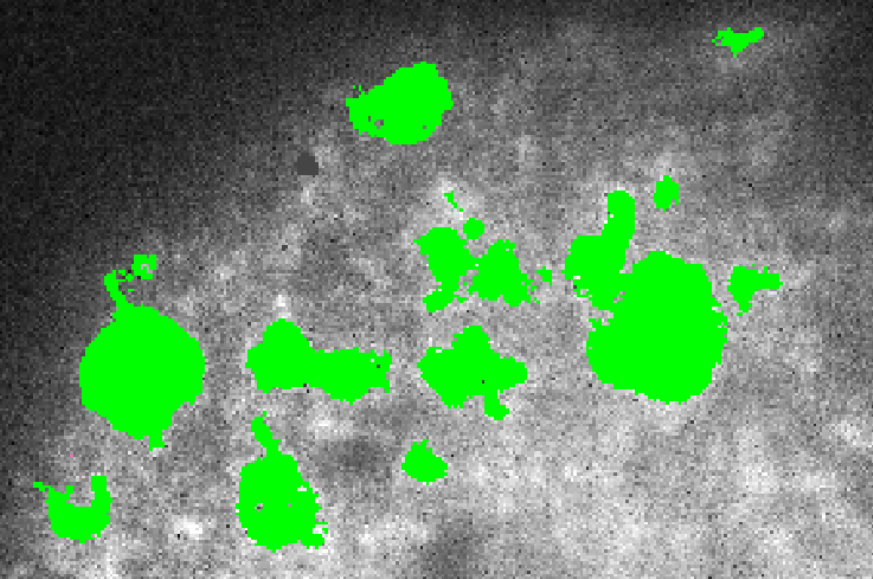
\includegraphics[width=0.7\textwidth]{images/gmm/data/A/dataA_false_positive.png}
    \caption[An excerpt of data set A - detections]{An excerpt of data set A
        (taken from~\citet{schiegg_13_conservation}): Detections are indicated by green color. A high
        false positive rate makes this data set challenging.}
    \label{fig:gmm-data-a-false-positive}
\end{figure}



\subsubsection{Data Set B - Drosophila Embryo past Gastrulation}
The second three-dimensional data set is another $3d+t$ recording of drosophila, but this time from
a later stage in the development of the embryo -- shortly after gastrulation. It is a time series of
100 volumes of the size $730 \times 320 \times 30$ with about 800 cells per frame. Due to the
advanced embryonic evolution, the cell population is much denser compared to data set
A~(\cref{fig:gmm-data-b-dense-population}). This increases the number of merged objects in the
segmentation~(\cref{fig:gmm-result-b} on Page~\pageref{fig:gmm-data-b-dense-population}) and therefore is
a demanding challenge fit to the capabilities of the conservation tracking.


\subsubsection{Data Set C - MitoCheck}
\label{subsubsec:gmm-data-c}
Finally, the third data set is a series of 92 $2d$ images with a resolution of $1344\times1024$,
publicly available on the website of the MitoCheck
project\footnote{\label{note1}\url{http://www.mitocheck.org/archive/cgi-bin/mtc?action=show_movie;query=87214}}. Due
to its two-dimensional nature, it contains merged objects caused not only by poor image quality but
also by occlusions. \cref{fig:gmm-data-c-three-slices} on Page~\pageref{fig:gmm-data-c-three-slices}
shows three frames of the data with an increasing number of cells and merged objects.





\begin{table}
    \centering
    \begin{tabularx}{\textwidth}{Xp{2cm}XX}
        \toprule
        Data set & Dimensions & Resolution & Challenge \\ \midrule
        A - Syncytial Blastoderm & $3d+t$ &  $40\times2362\times994\times47$& High false positive
        detection rate
        due to cytoplasm radiance \\
        B - Gastrulation & $3d+t$ & $100 \times 730 \times 320 \times 30$ & Many merged objects \\
        C - MitoCheck & $2d+t$ & $92\times1344\times1024$ & Many merged objects \\
        \bottomrule
    \end{tabularx}
    \caption[Data sets for evaluation of the conservation tracking]{Data sets for evaluation of the
        conservation tracking.}
    \label{tab:gmm-evaluation-data}
\end{table}

\subsection{Measures}
\label{subsec:gmm-measures}
In general, a tracking method is compared to ground truth for evaluation. Based on the \emph{true
    positive} events, \ie these events appear both in the experiment and ground truth, and the
\emph{false positive} and \emph{false negative} events, \ie these events appear in the experiment,
but not in the ground truth, and vice versa, we can define the performance measures
\emph{precision}, \emph{recall} and
\emph{$\fscore_\beta$-score}~\citep{powers_07_evaluation,makhoul_99_performance}. In the
following, $\tp$, $\fp$ and $\fn$ denote the numbers of true positives, false positives and false
negatives, respectively. Then, those three measures can be defined as
\begin{align}
    \precision &= \frac{\tp}{\tp+\fp} \in [0,1], \\
    \recall &= \frac{\tp}{\tp+\fn} \in [0,1], \\
    \fscore_\beta &= \left(1+\beta^2\right)\frac{\precision\cdot\recall}{\beta^2\precision+\recall} \in [0,1].
\end{align}
In a more descriptive way, precision and recall are the fractions of events in the experimental
results and ground truth, respectively, which were classified correctly. The weight $\beta$ in the
$\fscore_\beta$-score indicates the relative cost of false positives and false
negatives. Furthermore, with the commonly used setting $\beta=1$,
\begin{align}
    \fmeasure = 2\frac{\precision\cdot\recall}{\precision+\recall}
\end{align}
is the harmonic mean of precision and recall and indicates equal costs for Type-I and Type-II
errors. Naturally, a higher value of these measures reflects a better performance of a method. In
general, we set $\beta=1$ and use precision, recall and $\fmeasure$ for the evaluation of the
different event types listed in \cref{tab:gmm-events}.
\begin{table}
    \centering
    \begin{tabularx}{\textwidth}{lXl}
        \toprule
        \multicolumn{3}{l}{Event}  \\ \midrule
        Move & Cell $i$ at time $t$ is assigned to cell $j$ at time $t+1$. &
        \tikz[baseline=(t1.south),minimum size=58pt,scale=0.35, every node/.style={scale=0.35,
            text=black, font=\LARGE}, thick]{
            \begin{scope}
    \node (t1) {\huge $t$};
    \node[hypotheses_one_object, below=of t1.north, circle, draw,yshift=10mm] (x11) {$X_i^t$};
\end{scope}

\begin{scope}
    \node[right=of t1, xshift=-10mm] (t2) {\huge $t+1$};
    \node[hypotheses_one_object, below=of t2.north, circle, draw,yshift=10mm] (x21) {$X_j^{t+1}$};
\end{scope}

\path[hypothesestransition] (x11) edge (x21);

\begin{scope}[on background layer]
    \node[rectangle, draw, color=hypothesesbackground!40, fill=hypothesesbackground!30,
    fit=(x11), inner sep=4mm] (b1) {};
    \node[rectangle, draw, color=hypothesesbackground!40, fill=hypothesesbackground!30,
    fit=(x21), inner sep=4mm] (b2) {};
\end{scope}

%%% Local Variables: 
%%% mode: latex
%%% TeX-master: "../../../main"
%%% End: 

        }\\
        Division & Cell $i$ at time $t$ divides into cells $j$ and $h$ at time $t+1$. &
        \tikz[baseline=(t1.south),minimum size=58pt,scale=0.35, every node/.style={scale=0.35,
            text=black, font=\LARGE}, thick]{
            \begin{scope}
    \node (t1) {\huge $t$};
    \node[hypotheses_one_object, below=of t1.north, circle, draw,yshift=-2mm] (x11) {$X_i^t$};
\end{scope}

\begin{scope}[on background layer]
    \node[hypotheses_one_object, below=of t1.north, circle, draw,yshift=10mm] (x12) {$X_j^{t+1}$};
    \node[hypotheses_one_object, below=of t1.north, circle, draw,yshift=-21mm] (x13) {$X_h^{t+1}$};
\end{scope}

\begin{scope}
    \node[right=of t1, xshift=-10mm] (t2) {\huge $t+1$};
    \node[hypotheses_one_object, below=of t2.north, circle, draw,yshift=10mm] (x21) {$X_j^{t+1}$};
    \node[hypotheses_one_object, hypothesesdetection, below=of t2.north, circle, draw,yshift=-21mm] (x22) {$X_h^{t+1}$};
\end{scope}

\path[hypothesestransition] (x11) edge (x21);
\path[hypothesestransition] (x11) edge (x22);

\begin{scope}[on background layer]
    \node[rectangle, draw, color=hypothesesbackground!40, fill=hypothesesbackground!30,
    fit=(x12) (x13), inner sep=4mm] (b1) {};
    \node[rectangle, draw, color=hypothesesbackground!40, fill=hypothesesbackground!30,
    fit=(x21) (x22), inner sep=4mm] (b2) {};
\end{scope}


%%% Local Variables: 
%%% mode: latex
%%% TeX-master: "../../../main"
%%% End: 

        }\\
        Merger & Connected component $i$ at time $t+1$ is identified to be a merger of size $k$. In the example in
        the right column $k=2$.&
        \tikz[baseline=(t1.south),minimum size=58pt,scale=0.35, every node/.style={scale=0.35,
            text=black, font=\LARGE}, thick]{
            \begin{scope}
    \node (t2) {\huge $t$};
    \node[hypotheses_one_object, below=of t2.north, circle, draw,yshift=10mm] (x21) {$X_i^{t}$};
    \node[hypotheses_one_object, below=of t2.north, circle, draw,yshift=-21mm] (x22) {$X_h^{t}$};
\end{scope}

\begin{scope}
    \node[right=of t2, xshift=-10mm] (t1) {\huge $t+1$};
    \node[hypotheses_two_objects, below=of t1.north, circle, draw,yshift=-2mm] (x11) {$X_i^{t+1}$};
\end{scope}

\begin{scope}[on background layer]
    \node[hypothesesdetection, below=of t1.north, circle, draw,yshift=10mm] (x12) {$X_j^{t+1}$};
    \node[hypothesesdetection, below=of t1.north, circle, draw,yshift=-21mm] (x13) {$X_h^{t+1}$};
\end{scope}



\path[hypothesestransition] (x11) edge (x21);
\path[hypothesestransition] (x11) edge (x22);

\begin{scope}[on background layer]
    \node[rectangle, draw, color=hypothesesbackground!40, fill=hypothesesbackground!30,
    fit=(x12) (x13), inner sep=4mm] (b1) {};
    \node[rectangle, draw, color=hypothesesbackground!40, fill=hypothesesbackground!30,
    fit=(x21) (x22), inner sep=4mm] (b2) {};
\end{scope}


%%% Local Variables: 
%%% mode: latex
%%% TeX-master: "../../../main"
%%% End: 

        }\\
        Multiframe Move & Cell $i$ at time $t$ moves into a merged object at time $t+1$ and is
        identified as a single cell $j$ at time $t^{\prime}>t+1$.  &
        \tikz[baseline=(t1.south),minimum size=58pt,scale=0.35, every node/.style={scale=0.35,
            text=black, font=\LARGE}, thick]{
            \begin{scope}
    \node (t2) {\huge $t$};
    \node[hypotheses_one_object, below=of t2.north, circle, draw,yshift=10mm] (x21) {$X_l^{t}$};
    \node[hypotheses_one_object, below=of t2.north, circle, draw,yshift=-21mm] (x22) {$X_h^{t}$};
\end{scope}

\begin{scope}
    \node[right=of t2, xshift=-10mm] (t1) {\huge $t+1$};
    \node[hypotheses_two_objects, below=of t1.north, circle, draw,yshift=-2mm] (x11) {$X_i^{t+1}$};
\end{scope}

\begin{scope}[on background layer]
    \node[hypotheses_one_object, below=of t1.north, circle, draw,yshift=10mm] (x12) {$X_j^{t+1}$};
    \node[hypotheses_one_object, below=of t1.north, circle, draw,yshift=-21mm] (x13) {$X_h^{t+1}$};
\end{scope}

\begin{scope}
    \node[right=of t1, xshift=10mm] (t3) {\huge $t^{\prime}-1$};
    \node[hypotheses_two_objects, below=of t3.north, circle, draw,yshift=-2mm] (x31) {$X_m^{t^{\prime}-1}$};
\end{scope}

\begin{scope}[on background layer]
    \node[hypotheses_one_object, below=of t3.north, circle, draw,yshift=10mm] (x32) {$X_j^{t}$};
    \node[hypotheses_one_object, below=of t3.north, circle, draw,yshift=-21mm] (x33) {$X_h^{t+1}$};
\end{scope}

\begin{scope}
    \node[right=of t3, xshift=-10mm] (t4) {\huge $t^{\prime}$};
    \node[hypotheses_one_object, below=of t4.north, circle, draw,yshift=10mm] (x41) {$X_n^{t^{\prime}}$};
    \node[hypotheses_one_object, below=of t4.north, circle, draw,yshift=-21mm] (x42) {$X_j^{t^{\prime}}$};
\end{scope}

% \coordinate[xshift=8mm] at (x11.east) (c1);
% \coordinate[xshift=-8mm] at (x31.west) (c2);



\path[hypothesestransition] (x11) edge (x21);
\path[hypothesestransition] (x11) edge (x22);
\path[hypothesestransition] (x31) edge (x41);
\path[hypothesestransition] (x31) edge (x42);
\path[hypothesestransition, dashed] ($(x11.east)!0.2!(x31.west)$) edge ($(x11.east)!0.8!(x31.west)$);

\begin{scope}[on background layer]
    \node[rectangle, draw, color=hypothesesbackground!40, fill=hypothesesbackground!30,
    fit=(x12) (x13), inner sep=4mm] (b1) {};
    \node[rectangle, draw, color=hypothesesbackground!40, fill=hypothesesbackground!30,
    fit=(x21) (x22), inner sep=4mm] (b2) {};
    \node[rectangle, draw, color=hypothesesbackground!40, fill=hypothesesbackground!30,
    fit=(x32) (x33), inner sep=4mm] (b2) {};
    \node[rectangle, draw, color=hypothesesbackground!40, fill=hypothesesbackground!30,
    fit=(x41) (x42), inner sep=4mm] (b1) {};
\end{scope}


%%% Local Variables: 
%%% mode: latex
%%% TeX-master: "../../../main"
%%% End: 

        }\\ \bottomrule
    \end{tabularx}

%%% Local Variables: 
%%% mode: latex
%%% TeX-master: "../../../main"
%%% End: 

    \caption[Events in the conservation tracking]{Events for evaluation in the conservation tracking
        experiment. Note that a correct classification of a division requires not only that the
        parent cell is detected, but also the correct child cells. Furthermore, a merger event is
        only classified correctly if the correct number of objects has been inferred.}
    \label{tab:gmm-events}
\end{table}

\subsection{Results}
\label{subsec:gmm-results}
In this section we evaluate the performance of our proposed method on the data sets presented in
\cref{subsec:gmm-data}. Based on the measures defined in \cref{subsec:gmm-measures} we compare our
method to the state of the art tracking-by-assignment algorithm by \citet{kausler_12_discrete}.  In
addition to the evaluation of the tracking, we show the stand-alone performance of the division and
cell classifiers, where applicable. For the division classifier evaluation, contrary to the
evaluation of divisions in the tracking result, the correct classification of a mitotic cell, \ie a
cell that will divide in the subsequent time step, is sufficient.


\begin{table}
    \centering\small
    \begin{tabularx}{\textwidth}{c||c|cccc|cccc}
        \toprule
        & A & \multicolumn{4}{c|}{B} &
        \multicolumn{4}{c}{C} \\ 
        Parameter& $m=1$ & $m=1$ & $m=2$ & $m=3$ & $m=4$ & $m=1$ & $m=2$ & $m=3$ & $m=4$\\ \hline\small
        $\alpha$ & $25$ &5&5&5&5&5&5&5&5\\
        $w_{\text{app}}$ & $50$ &50&100&100&100&100&100&100&100\\
        $w_{\text{dis}}$ & $50$ &100&100&100&100&100&100&100&100\\
        $w_{\text{tr}}$ & $13$ &33&22&22&24&10&10&10&10\\
        $w_{\text{div}}$ & $28$ &40&26&41&36&36&16&16&16\\
        \bottomrule
    \end{tabularx}
    \caption[Conservation tracking - parameter settings]{Parameter settings for the conservation
        tracking in the experiments for data sets A, B and C~(\cref{subsec:gmm-data}). In all cases,
    the parameters were determined in an exhaustive grid search.}
    \label{tab:gmm-experiments-parameters}
\end{table}

\subsubsection{Data Set A -  Drosophila Embryo in Syncytial Blastoderm}
\label{subsubsec:gmm-reults-data-a}
For the comparison of the methods on data set A, we apply both tracking algorithms to a published
segmentation. This segmentation contains many false positive detections due to noise and
no merged objects~(\cref{fig:gmm-data-a-false-positive}). Therefore, we set the maximum number of
objects per connected component, model parameter $m$, to one. Furthermore, we use the same
classifier for detected cell as \citet{kausler_12_discrete}.

We obtain the optimal parameter settings~(\cref{tab:gmm-experiments-parameters}) in a grid
search. The tracking results are then evaluated based on precision, recall and
$\fmeasure$~(\cref{tab:gmm-experiments-data-a-results}). Our method yields comparable results
($\fmeasure=0.94$ and $\fmeasure=0.90$ on moves and divisions respectively) with
\citet{kausler_12_discrete} performing marginally better ($\fmeasure=0.96$ for moves and
$\fmeasure=0.92$ for divisions). The slightly better performance of \citet{kausler_12_discrete} can
be explained by their exploitation of the cell cycle
duration~\citep[Figure~5b]{kausler_12_discrete}.

\begin{table}
\centering
% \scalebox{0.8} {
\begin{tabular}{l||ccc|ccc}
    \toprule
							& \multicolumn{3}{c|}{\textbf{Overall:} 12,289 } & \multicolumn{3}{c}{\textbf{Divisions:} 380 }  \\
							& Precision & Recall & $\fmeasure$ &
                                                        Precision & Recall & $\fmeasure$    \\
\hline
\citet{kausler_12_discrete}& 0.96& 0.96 & 0.96  & 0.92     & 0.91 & 0.92    \\
Classifiers only*				        & \textit{N/A}   & \textit{N/A} & \textit{N/A} & 0.79 & 0.69 & 0.74 \\
Ours ($m=1$)						& 0.94        & 0.95 & 0.94  & 0.92      &
0.88 & 0.90   \\
\bottomrule
% /export/home/mschiegg/software/embryonic/toolbox/multitrack_ilastik06 --method=conservation --max-number-objects=1 --min-size=3 --max-neighbor-distance=100 --division-threshold=0.1 --z-scale=12.3 --ext-probs=/export/home/mschiegg/iccv2013/hufnagel2011/detProbs/%02d.h5 --ep_gap=0.0 --div=28 --tr=13 --app=50 --dis=50 --trans-par=25 --border-width=0 -o /export/home/mschiegg/iccv2013/hufnagel2011/paraopt/m=1/core0/ /export/home/mschiegg/iccv2013/hufnagel2011/conservationTracking_2013-08-23.ilp && /export/home/mschiegg/software/embryonic/toolbox/compare_tracking --quietly /export/home/mschiegg/iccv2013/hufnagel2011/manual_tracking_sorted2/ /export/home/mschiegg/iccv2013/hufnagel2011/paraopt/m=1/core0/
\end{tabular} 
% } % scalebox
%\vspace{-0.05cm}
\caption[Conservation tracking results: Data Set A]{Cell tracking results for data set A~(taken and
    modified from \citealp{schiegg_13_conservation}). Precision,
recall and $\fmeasure$-score measure the performance of both tracking algorithms compared to ground truth.}.
\label{tab:gmm-experiments-data-a-results}
\end{table}

\subsubsection{Data Set B - Drosophila Embryo past Gastrulation}
\begin{figure}
    \centering
    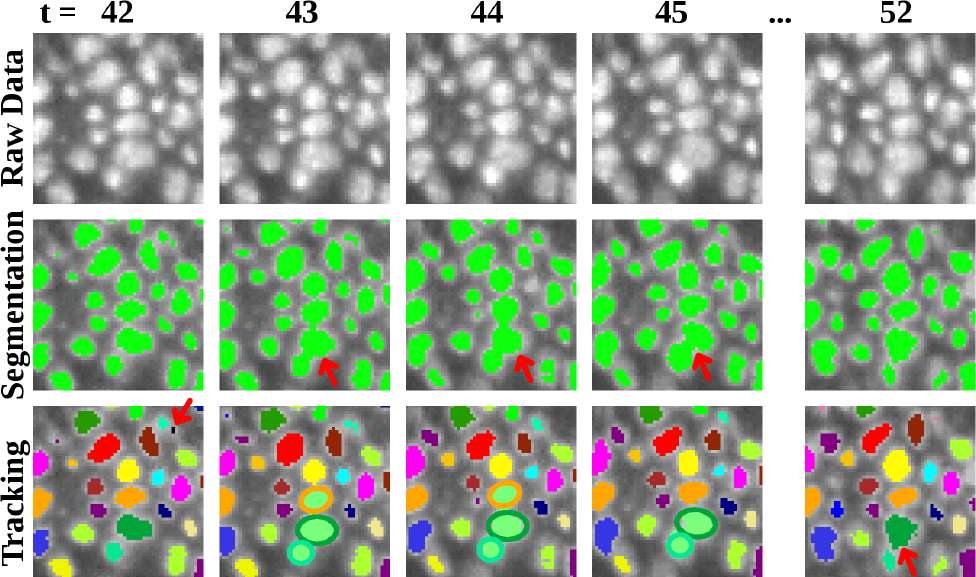
\includegraphics[width=\textwidth]{images/gmm/results/B/result_with_demerging.png}
    \caption[Excerpt of data set A: raw data, segmentation and tracking result]{A short time
        sequence of $2d$ images extracted from the $3d+t$ data set B of a drosophila embryo shortly
        after gastrulation~(taken from \citealp{schiegg_13_conservation}). The first row shows the raw
        data, followed by the segmentation in the middle row and, finally, the tracking result in
        the bottom row. Segmentation errors that stem from multiple objects being detected as a
        single connected component~(undersegmentation) are indicated by red arrows in the middle
        row. Moreover, the red arrow at $t=42$ in the bottom row shows an oversegmentation error that has been
        disabled by the tracking as indicated by black color. In the bottom row, the ellipses in
        time steps $43$-$45$ represent Gaussian mixture models that were fit to the detected merged
        connected components with the appropriate number of components. Our model is capable of
        reproducing the cell identities over a long time range ($42$-$52$), even if the merger
        configuration changes over time~(the addressed connected components contain three cells in
        time steps $43$ and $42$, and two cells at time $44$).}
    \label{fig:gmm-result-b}
\end{figure}
In the second data set B, the cell population is much denser compared to data set A. As a result,
the segmentation~\citep{sommer_11_ilastik} contains many merged
objects~(\cref{fig:gmm-result-b}). While these undersegmentation errors cannot be handled by
\citet{kausler_12_discrete}, our method makes use of its merger detection and cell reconstruction
capabilities~(\cref{tab:gmm-result-b}).

The tracking results are evaluated with respect to ground truth that has been generated
manually. \cref{tab:gmm-result-b} summarizes these results on data set B. Naturally,
\citep{kausler_12_discrete} cannot produce results for merged objects as they do not model multiple
objects per connected component. However, as shown in \cref{fig:gmm-result-b}, resolving merged
objects is vital for competitive tracking result in this data set. This is reflected by our method
outperforming the method in \citet{kausler_12_discrete}, \eg for divisions, they achieve an
$\fmeasure$-score of $0.06$ compared to our model's $0.71$. In addition to an accurate detection of
the correct number of objects in a connected component (precision$=0.78$), our model can resolve the
identities of these merged objects and reproduce moves over multiple frames with an
$\fmeasure$-score of $0.67$. Note that evaluation of multiframe moves is not conditioned on the
correct detections and transitions of mergers. Thus, an error in the detection of a merger will
automatically degrade the performance of the multiframe move reconstruction.

\begin{table}
    % \small
    % \hfill{}
    \centering
    \begin{tabular}{l||ccc|ccc}
        \toprule
        & \multicolumn{3}{c|}{\textbf{Moves}} & \multicolumn{3}{c}{\textbf{Divisions}}  \\
        & Precision & Recall & $F_1$& Precision& Recall& $F_{1}$\\
        \hline
        \citep{kausler_12_discrete} 	& 0.92		& 0.92 & 0.92  & 0.05      & 0.12 & 0.06    \\
        Classifiers only 	& \textit{N/A}	& \textit{N/A} & \textit{N/A}  & 0.83      & 0.64 & 0.72    \\
        Ours ($m=1$)						& 0.97        & 0.95 & 0.96  & 0.62     & 0.63 & 0.63    \\  
        Ours ($m=2$)						& 0.97        & 0.97 & 0.97  & 0.53      & 0.79 & 0.64   \\ 
        Ours ($m=3$)						& 0.97        & 0.97 & 0.97  & 0.70      & 0.76 & 0.73    \\ 
        Ours ($m=4$)						& 0.97        & 0.97 & 0.97  & 0.65      & 0.77 & 0.71    \\ 
        \midrule
        & \multicolumn{3}{c|}{\textbf{Mergers} } & \multicolumn{3}{c}{\textbf{Resolved Mergers}} \\
        & Precision& Recall& $F_{1}$ & Precision& Recall& $F_{1}$ \\
        \hline
        \citep{kausler_12_discrete} & \textit{N/A}& \textit{N/A} & \textit{N/A} & \textit{N/A}& \textit{N/A} & \textit{N/A} \\
        Classifiers only & 0.63 & 0.31 & 0.41 & \textit{N/A}& \textit{N/A} & \textit{N/A} \\
        Ours ($m=1$) & \textit{N/A}& \textit{N/A} & \textit{N/A} & \textit{N/A}& \textit{N/A} & \textit{N/A}\\
        Ours ($m=2$) & 0.71 & 0.54 & 0.61 & 0.72 & 0.61 & 0.66 \\
        Ours ($m=3$) & 0.73 & 0.58 & 0.64  & 0.73      & 0.63 & 0.67 \\
        Ours ($m=4$) & 0.78      & 0.59 & 0.67 & 0.74      & 0.63 & 0.60 \\
        \bottomrule
    \end{tabular}
    \caption[Conservation tracking results: Data Set B]{Evaluation of the performance on data set
        B~(taken and modified from \citealp[Table~2]{schiegg_13_conservation}). The tracking results
        are evaluated with regard to manually generated ground truth.}
    \label{tab:gmm-result-b}
\end{table}


Another building block for the success of our model on this data set is the use of the probabilistic
division prior $\phi_{\text{div}}$ that -- by itself -- reaches an $\fmeasure$-score of $0.72$ for
predicting mitotic cells. In order to give an overview of the tracking result and also to show the
complexity of cell tracking, \cref{fig:gmm-result-b-projection} shows a $2d$ projection of the $3d$
trajectories of cells in data set B.

\begin{figure}
    \centering
    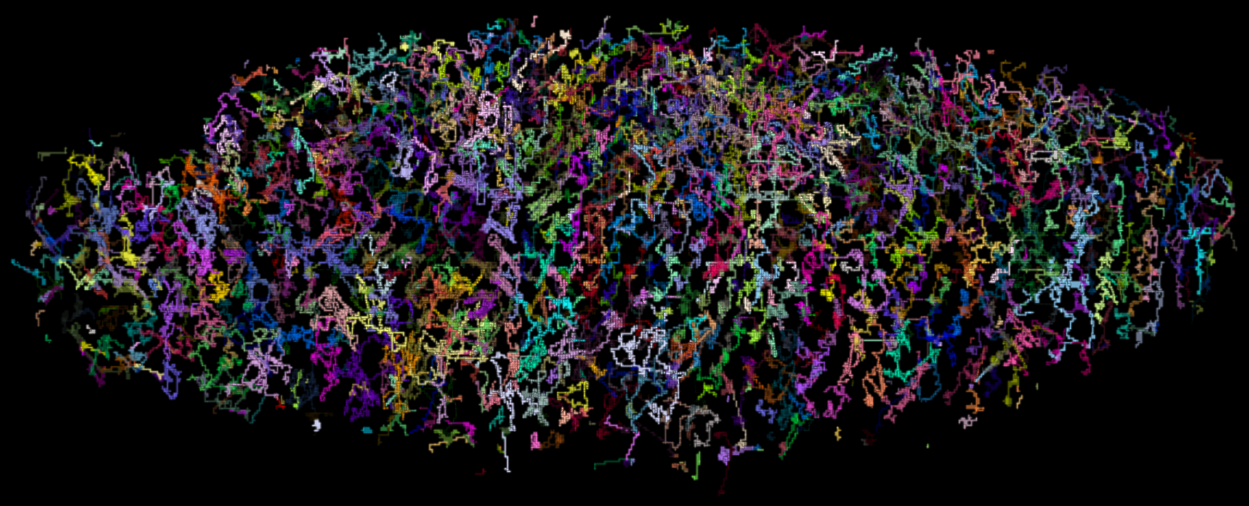
\includegraphics[width=\textwidth]{images/gmm/results/B/projection.png}
    \caption[$2d$ projection of trajectories in data set B]{$2d$ projection of the $3d$ trajectories of cells in data set B~(taken from
        \citealp{schiegg_13_conservation}): Colors encode individual cells. In case of divisions,
        both child cells take the color of their ancestor cell.}
    \label{fig:gmm-result-b-projection}
\end{figure}



\subsubsection{Data Set C - MitoCheck}
\def\imagetop#1{\vtop{\null\hbox{#1}}}
\newlength\tablemathtext
\settototalheight\tablemathtext{\parbox{\linewidth}{$t=75$, $\id=446$}}
\begin{table}
    \centering
    \scalebox{0.85}{
        \def\arraystretch{0.5}
% \setlength{\tabcolsep}{1pt}
\begin{tabular}{lccc}
    \toprule
    Time Step \& Id  & Raw Data & Segmentation & GMM fit \\ \midrule
    % \begin{minipage}[t]{0.15\linewidth}\small\vspace{-53pt}{$\begin{aligned}t&=75\\\id&=446\\
    %         k&=3\end{aligned}$}\end{minipage}&
    % \raisebox{-0.8\height{\includegraphics...}}
    $t=75$, $\id=446$&
    \raisebox{\tablemathtext-\height}{
        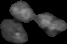
\includegraphics[width=0.18\textwidth]{images/gmm/gmm_2d_fit/t=75,id=446,k=3_raw.png}} &
    \raisebox{\tablemathtext-\height}{
        
\includegraphics[width=0.18\textwidth]{images/gmm/gmm_2d_fit/t=75,id=446,k=3_label.png}} &
    \raisebox{\tablemathtext-\height}{
        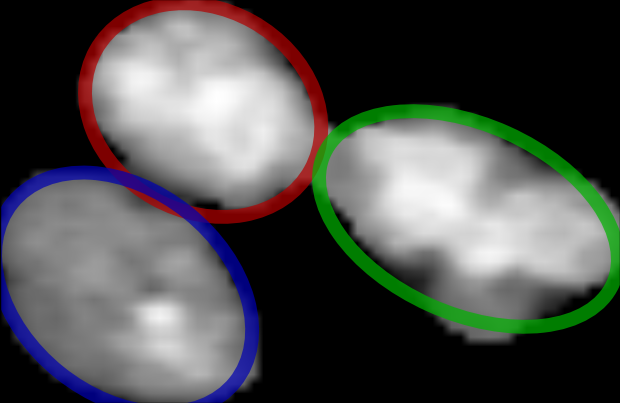
\includegraphics[width=0.18\textwidth]{images/gmm/gmm_2d_fit/t=75,id=446,k=3_fit.png}} \\
    &&& \\
    $t=85$, $\id=12$&
    \raisebox{\tablemathtext-\height}{
        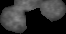
\includegraphics[width=0.18\textwidth]{images/gmm/gmm_2d_fit/t=85,id=12,k=3_raw.png}} &
    \raisebox{\tablemathtext-\height}{
        
\includegraphics[width=0.18\textwidth]{images/gmm/gmm_2d_fit/t=85,id=12,k=3_label.png}} &
    \raisebox{\tablemathtext-\height}{
        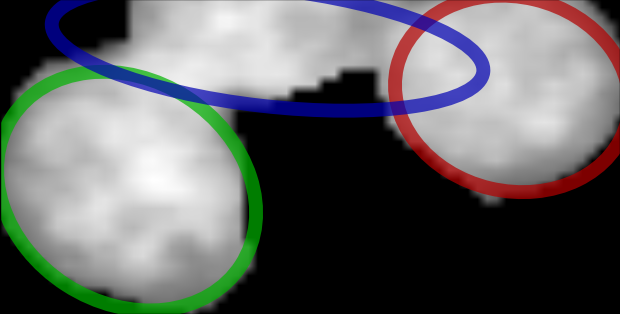
\includegraphics[width=0.18\textwidth]{images/gmm/gmm_2d_fit/t=85,id=12,k=3_fit.png}} \\
    &&& \\
    $t=75$, $\id=206$&
    \raisebox{\tablemathtext-\height}{
        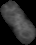
\includegraphics[width=0.18\textwidth]{images/gmm/gmm_2d_fit/t=75,id=206,k=2_raw.png}} &
    \raisebox{\tablemathtext-\height}{
        
\includegraphics[width=0.18\textwidth]{images/gmm/gmm_2d_fit/t=75,id=206,k=2_label.png}} &
    \raisebox{\tablemathtext-\height}{
        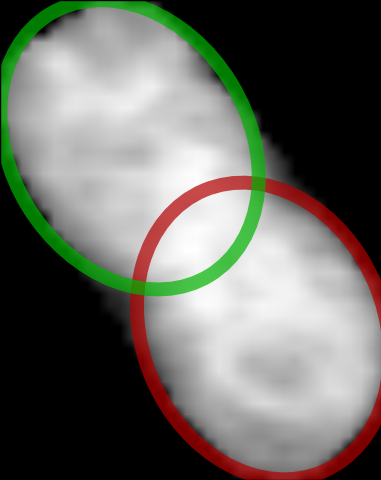
\includegraphics[width=0.18\textwidth]{images/gmm/gmm_2d_fit/t=75,id=206,k=2_fit.png}} \\
    % &
    % \raisebox{\tablemathtext-\height}{
\includegraphics[width=0.18\textwidth]{images/gmm/gmm_2d_fit/t=50,id=198,k=3_raw.png}} &
    % \raisebox{\tablemathtext-\height}{
\includegraphics[width=0.18\textwidth]{images/gmm/gmm_2d_fit/t=50,id=198,k=3_label.png}} &
    % \raisebox{\tablemathtext-\height}{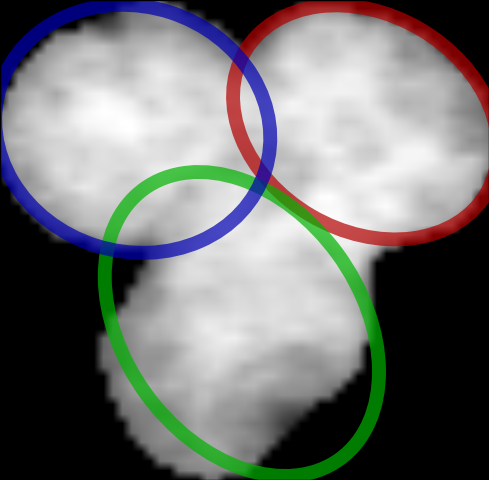
\includegraphics[width=0.18\textwidth]{images/gmm/gmm_2d_fit/t=50,id=198,k=3_fit.png}} \\ &
    &&& \\
    $t=75$, $\id=446$&
    \raisebox{\tablemathtext-\height}{
        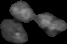
\includegraphics[width=0.18\textwidth]{images/gmm/gmm_2d_fit/t=75,id=446,k=3_raw.png}} &
    \raisebox{\tablemathtext-\height}{
\includegraphics[width=0.18\textwidth]{images/gmm/gmm_2d_fit/t=75,id=446,k=3_label.png}} &
    \raisebox{\tablemathtext-\height}{
        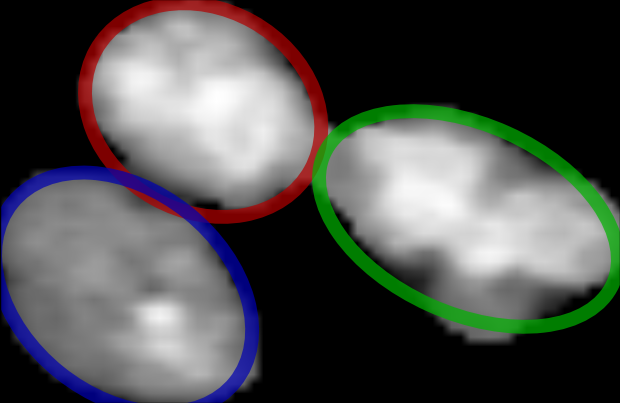
\includegraphics[width=0.18\textwidth]{images/gmm/gmm_2d_fit/t=75,id=446,k=3_fit.png}} \\
    &&& \\
    $t=50$, $\id=122$&
    \raisebox{\tablemathtext-\height}{
        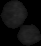
\includegraphics[width=0.18\textwidth]{images/gmm/gmm_2d_fit/t=50,id=122,k=2_raw.png}} &
    \raisebox{\tablemathtext-\height}{
\includegraphics[width=0.18\textwidth]{images/gmm/gmm_2d_fit/t=50,id=122,k=2_label.png}} &
    \raisebox{\tablemathtext-\height}{
        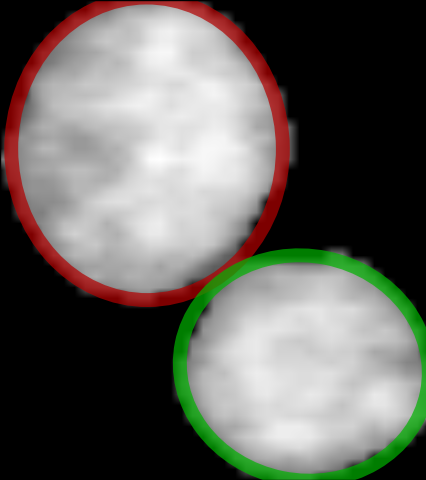
\includegraphics[width=0.18\textwidth]{images/gmm/gmm_2d_fit/t=50,id=122,k=2_fit.png}} \\
    &&& \\
    $t=85$, $\id=334$&
    \raisebox{\tablemathtext-\height}{
        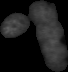
\includegraphics[width=0.18\textwidth]{images/gmm/gmm_2d_fit/t=85,id=334,k=4_raw.png}} &
    \raisebox{\tablemathtext-\height}{
        \hspace{-3pt}
\includegraphics[width=0.18\textwidth]{images/gmm/gmm_2d_fit/t=85,id=334,k=4_label.png}} &
    \raisebox{\tablemathtext-\height}{
        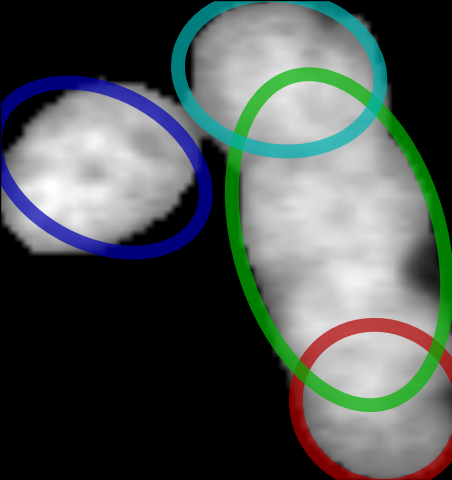
\includegraphics[width=0.18\textwidth]{images/gmm/gmm_2d_fit/t=85,id=334,k=4_fit.png}} \\
    \bottomrule
\end{tabular}
\def\arraystretch{1.0}

% WHY THE FUCK THE NEED FOR NEGATIVE HSPACE IN LAST ROW?

%%% Local Variables: 
%%% mode: latex
%%% TeX-master: "../../../../main"
%%% End: 

    }
    \caption[GMM fits to two-dimensional cells]{\small GMM fits to two-dimensional cells from data set
        C: Based on the inferred number of cells per connected components, the rightmost column
        shows GMM fits to the bounding box images of merged objects with ids $\id$ at times $t$ as an overlay
        on the raw data. Here, the ellipses represent covariances of mixture components, centered
        add the corresponding means. Note that
        column two shows the connected components in their original intensity range, whereas the intensity
        has been stretched to $[0,255]$ in the rightmost column in the process of overlaying the
        fit. Furthermore, partial objects in the segmentation, which are not objects of interest, are not
        displayed. The second row shows a merged object that has been cut off by the image border. Still,
        conservation tracking manages to infer the correct number of cells and the GMM fit yields a
        reasonable estimate on the region centers of the individual objects.}
   \label{tab:gmm-results-c-fits}
\end{table}

Data set C completes our evaluation of the model. Again, a gold standard for evaluation has been
acquired manually. Other than the data sets above, data set C has only two spatial dimensions, which
necessarily leads to merged objects caused by occlusion, even if the image quality is
good~(\cref{fig:gmm-data-c-three-slices,tab:gmm-results-c-fits}). This time, the merger classifiers
perform weakly, but the conservation tracking graphical model boosts this result. In general, with
an active merger detection, \ie $m>1$, our approach outperforms the method of
\citet{kausler_12_discrete}. \cref{tab:gmm-result-c} summarizes the results for four different
settings of the parameter $m$, which specifies the maximum possible number of objects per connected
component.
%In addition, \cref{tab:gmm-number-of-merged-objects} shows the number of merged objects
%inferred by our method for both data set B and data set C.

\begin{table} % \small % \hfill{} \centering
    \begin{tabular}{l||ccc|ccc}
        \toprule
        & \multicolumn{3}{c|}{\textbf{Moves}} & \multicolumn{3}{c}{\textbf{Divisions}} \\
        & Precision& Recall& $\fmeasure$ & Precision& Recall& $\fmeasure$ \\ \hline
        \citep{kausler_12_discrete} & 0.99 & 0.97 & 0.98 & 0.65 & 0.68 & 0.66 \\
        Classifiers only & \textit{N/A} & \textit{N/A} & \textit{N/A} & 0.92 & 0.56 & 0.70 \\
        Ours ($m=1$) & 0.99 & 0.97 & 0.98 & 0.68 & 0.71 & 0.70 \\
        Ours ($m=2$) & 1.00 & 0.99 & 0.99 & 0.85 & 0.76 & 0.80 \\
        Ours ($m=3$) & 1.00 & 0.99 & 0.99 & 0.85 & 0.77 & 0.80 \\
        Ours ($m=4$) & 1.00 & 0.99 & 0.99 & 0.85 & 0.76 & 0.80 \\
        \midrule & \multicolumn{3}{c|}{\textbf{Mergers} } & \multicolumn{3}{c}{\textbf{Resolved Mergers}} \\ 
        & Precision& Recall& $F_{1}$ & Precision& Recall& $F_{1}$ \\ \hline
        \citet{kausler_12_discrete} & \textit{N/A}& \textit{N/A} & \textit{N/A} & \textit{N/A}&
        \textit{N/A} & \textit{N/A} \\
        Classifiers only & 0.41 & 0.62 & 0.49 & \textit{N/A}& \textit{N/A} & \textit{N/A} \\
        Ours ($m=1$) & \textit{N/A}& \textit{N/A} & \textit{N/A} & \textit{N/A}& \textit{N/A} & \textit{N/A}\\ 
        Ours ($m=2$) & 0.73 & 0.60 & 0.66 & 0.79 & 0.70 & 0.74\\
        Ours ($m=3$) & 0.84 & 0.69 & 0.76 & 0.85 & 0.75 & 0.79\\
        Ours ($m=4$) & 0.84 & 0.69 & 0.76 & 0.85 & 0.75 & 0.80\\
        \bottomrule
    \end{tabular}
    \caption[Conservation tracking results: Data Set C]{Evaluation of the performance on data set
C~(taken and modified from \citealp[Table~2]{schiegg_13_conservation}). The tracking results are
evaluated with regard to manually generated ground truth.}
    \label{tab:gmm-result-c}
\end{table}


Again, the set of optimal parameters as shown in \cref{tab:gmm-experiments-parameters} has been
determined by a grid search over a range of 720 parameters, which also allows for an evaluation of
the sensitivity to parameter changes of our model. To that end, \cref{fig:gmm-results-c-vis-sensitivity}
plots the $\fmeasure$ performances for each parameter setting. Naturally, with a high number of
unambiguous moves in data set C, the overall $\fmeasure$-score is not affected by the choice of
parameters. Even though there are a couple of outlier parameter settings that perform badly for
divisions, the method is fairly robust to variation of the parameter settings.
% \begin{table}
%     \centering
%     \begin{tabular}{l||ccc|ccc}
%         \toprule
%         &\multicolumn{3}{c|}{\textbf{Data Set B}}&\multicolumn{3}{c}{\textbf{Data Set B}} \\
%         & $(2)$ & $(3)$ & $(4)$ & $(2)$ & $(3)$ & $(4)$ \\ \hline
%         Ours $(m=2)$ & 979 & \textit{N/A} & \textit{N/A} &&& \\
%         Ours $(m=3)$ & 859 & 116 & \textit{N/A} &&& \\
%         Ours $(m=4)$ & 859 & 115 & 1 &&& \\
%         Ground Truth & 987 & 156 & 48 &&& \\
%         \bottomrule
%     \end{tabular}
%     \caption{Number of merged objects per connected component in data sets B and C.}
%     \label{tab:gmm-number-of-merged-objects}
% \end{table}
\begin{figure}
    \centering
    \begin{subfigure}[t]{0.48\textwidth}
        \centering
        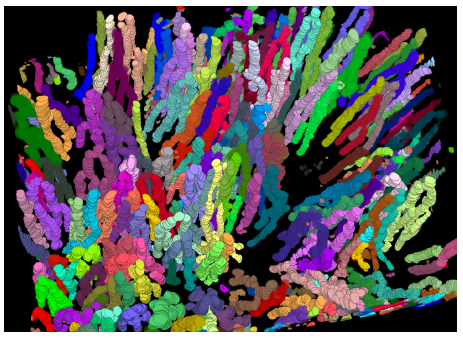
\includegraphics[width=\textwidth]{images/gmm/results/C/space_time_rendering.png}
        \caption{Space-time rendering of the conservation tracking result~(taken from
            \citealp[Figure~6c]{schiegg_13_conservation}).}
        \label{fig:gmm-results-c-visualization}
    \end{subfigure}
    \hfill
    \begin{subfigure}[t]{0.48\textwidth}
        \centering
        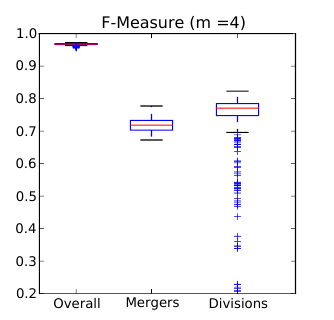
\includegraphics[width=0.828\textwidth]{images/gmm/results/C/sensitivity.png}
        \caption{Parameter sensitivity of the $\fmeasure$ performance on the overall tracking as
            well as on merger and division events for our method on data set C~(taken from
            \citealp[Figure~6d]{schiegg_13_conservation}).}
        \label{fig:gmm-results-c-sensitivity}
    \end{subfigure}
    \caption[Visualization of the tracking results for data set C and parameter sensitivity]{The
        tracking result of our method is visualized in~(\subref{fig:gmm-results-c-visualization}) in
        terms of a space-time rendering the trajectories of the cells with each color indicating a
        unique track. Children cells inherit the color of their ancestor and divisions are clearly
        visible as forks of tracks into two branches of the same color. The parameter
        sensitivity evaluation (\subref{fig:gmm-results-c-sensitivity}) shows that our method is
        fairly robust towards a change in parameter settings.}
    \label{fig:gmm-results-c-vis-sensitivity}
\end{figure}




Finally, the results of the classifier evaluation in \cref{tab:gmm-result-c} show that global
information embedded in a graphical model give a strong boost to the comparibly weak performance of
the local merger classifiers.

In this chapter we introduced a cell reconstruction method for conservation tracking based on
Gaussian mixture models. In the experimental evaluation, conservation tracking performs comparably to
the state of the art method, chain graph tracking~(\cref{subsec:fg-chaingraph}), in a merger-free
setting. Furthermore, conservation tracking is able to reliably detect merged objects and
reconstruct unique tracks. Still, tracking results are highly dependent on the segmentation. To
address this, we present a joint segmentation and tracking method in \cref{cha:joint}, which breaks
the barrier between segmentation and tracking in the context of tracking-by-assignment.

% After the extensive discussion of our proposed model for cell identity reconstruction in the context
% of the conersvation tracking, both in theory and experiments, the following ~\cref{cha:joint} will
% be dedicated to the introduction of a new graphical model based method which breaks the barrier
% between segmentation and tracking.



%%% Local Variables: 
%%% mode: latex
%%% TeX-master: "../../../main"
%%% End: 




%%% Local Variables: 
%%% mode: latex
%%% TeX-master: "../../main"
%%% End: 
